% (c) 2012 Tiziana Manca - tmanca@libero.it
% (c) 2012 Silvia Cibola - silvia.cibola@gmail.com
% (c) 2012-2014 Dimitrios Vrettos - d.vrettos@gmail.com
% (c) 2014 Daniele Zambelli - daniele.zambelli@gmail.com

%===================================
\section{Esercizi}
%===================================
\subsection{Esercizi dei singoli paragrafi}
%===================================
%\subsubsection*{B.1 - Proposizioni e predicati}
\subsubsection*{\numnameref{sec:proposizioni}}

\begin{esercizio}
\label{ese:B.1}
Completa la tabella come suggerito nella prima riga, individuando, per 
ciascuna proposizione, il predicato e gli argomenti a cui esso si riferisce:
\begin{center}
\begin{tabular}{llc}
\toprule
Proposizioni & Predicato & Argomenti\\
\midrule
7 è divisore di~14 & essere divisore di & 7, 14 \\
11 è maggiore di~10 & essere maggiore di & \\
5 è numero primo & & \\
Andrea frequenta la stessa palestra di Marco & & \\
Marta è moglie di Piero & & \\
Paolo è padre di Marco & & \\
\bottomrule
\end{tabular}
\end{center}
\end{esercizio}

\begin{comment}
 
%\subsubsection*{C.2 - Rappresentazione di una corrispondenza}
\subsubsection*{\numnameref{sec:corrispondenze}}

\begin{esercizio}
\label{ese:C.1}
Rappresenta con un grafico cartesiano la corrispondenza~$\Kor$: "essere nato 
nell'anno" di dominio l'insieme~$A=$ \{Galileo, Napoleone, Einstein, Fermi, 
Obama\}
e codominio l'insieme~$B=$\{1901, 1564, 1961, 1879, 1769, 1920, 1768\}. 
Rappresenta per elencazione il sottoinsieme~$G_\Kor$ del prodotto cartesiano~$A 
\times B$
Stabilisci infine gli elementi dell'immagine~$\IM$
\end{esercizio}

\begin{esercizio}
\label{ese:C.2}
L'insieme~$S=$ \{casa, volume, strada, ufficio, clavicembalo, cantautore, 
assicurazione\} è il codominio della corrispondenza~$\Kor$: "essere il numero di 
sillabe di" il cui dominio
è~$X=\{x \in\insN / 0<x<10\}$ Rappresenta con un grafico cartesiano la 
corrispondenza assegnata, evidenzia come nel primo esempio di questo paragrafo 
l'insieme~$G_\Kor$,
scrivi per elencazione l'insieme~$\IM$
\end{esercizio}

\begin{esercizio}
\label{ese:C.3}
Completa la rappresentazione con grafico sagittale della corrispondenza "essere 
capitale di". La freccia che collega gli elementi del dominio con quelli del 
codominio rappresenta
il predicato~$\Kor$: "essere la capitale di".
\begin{center}
 % (c) 2012 Dimitrios Vrettos - d.vrettos@gmail.com
\begin{tikzpicture}[font=\small,x=10mm, y=5mm]

\draw[->] (0,0) -- (8,0) node [below right] () {$r$};
\node[above]  at (4,0) {$2$};
\begin{scope}[blue,thick,->]
\draw (4,0) -- (8,0);
\draw[fill=blue] (4,0)circle (1.5pt);
\end{scope}

\end{tikzpicture}
\end{center}

\end{esercizio}

% %\subsubsection*{C.3 - Caratteristiche di una corrispondenza}
% %\subsubsection*{\numnameref{sec:C_caratteristiche}}
% 
% \begin{esercizio}
% \label{ese:C.4}
% È univoca la corrispondenza~$\Kor$ definita tra l'insieme~$P=$ \{parola del 
% proverbio "rosso di sera, bel tempo si spera"\} e l'insieme~$A=$\{lettere 
% dell'alfabeto italiano\}
% che associa ad ogni parola la sua iniziale? Ti sembra corretto affermare che 
% dominio e insieme di definizione coincidono? Completa con il simbolo corretto
% la relazione tra insieme immagine e codominio:~$\IM\ldots\Cod$ Fai il grafico 
% sagittale della corrispondenza.
% \end{esercizio}
% 
% \begin{esercizio}
% \label{ese:C.5}
% $\Kor$ è la corrispondenza tra l'insieme ~$\insN$ dei naturali e l'insieme 
% degli interi relativi~$\insZ$ espressa dal predicato "essere il quadrato di". Ti 
% sembra corretto affermare che
% dominio e insieme di definizione coincidono? Perché~$\IM=\Cod$? La 
% corrispondenza è univoca?
% \end{esercizio}
% % \newpage
% \begin{esercizio}
% \label{ese:C.6}
% Una corrispondenza~$\Kor$ è assegnata con il suo grafico cartesiano.
% \begin{center}
%  % (c) 2012 Dimitrios Vrettos - d.vrettos@gmail.com
\begin{tikzpicture}[font=\small,x=10mm, y=5mm]

\draw[->] (0,0) -- (8,0) node [below right] () {$r$};
\node[above]  at (2,0) {$-2$};
\node[above]  at (6,0) {2};
\begin{scope}[blue,thick]
\draw (2,0) -- (6,0);
\foreach \x in {2,6}
\draw[fill=white] (\x,0)circle (1.5pt);
\end{scope}

\end{tikzpicture}
% \end{center}
% Completa e rispondi alle domande:
% 
% \begin{enumeratea}
% \item $\Dom=$\{\dotfill\};
% \item $\Cod=$\{\dotfill\};
% \item $\ID=$\{\dotfill\};
% \item $\IM=$\{\dotfill\};
% \item la corrispondenza è biunivoca?
% \item 2 è l'immagine di quali elementi dell'insieme di definizione?
% \item quale elemento del codominio è l'immagine di~$M$?
% \end{enumeratea}
% \end{esercizio}
% 
% % \newpage
% \begin{esercizio}
% \label{ese:C.7}
% I tre grafici sagittali rappresentano altrettante corrispondenze, $\Kor_1$, 
% $\Kor_2$, $\Kor_3$
% Completa per ciascuna di esse la descrizione schematizzata nel riquadro 
% sottostante:
% \begin{center}
%  % (c) 2012 Dimitrios Vrettos - d.vrettos@gmail.com
\begin{tikzpicture}[x=10mm, y=10mm]

\node[circle, minimum height=2cm,draw] (A) at (0,0) {};

\node[above] (A1) at (A.north) {$A$};

\begin{scope}[fill=CornflowerBlue]

\filldraw (.5,.5) circle (2pt) node (a) {};
\node[left] at (.5,.5) {1};
\filldraw (.8,.2) circle (2pt) node (b) {};
\node[left] at (.8,.2) {2};
\filldraw (-.4,-.5) circle (2pt) node (c) {};
\node[left] at (-.4,-.5)  {3};
\filldraw (-.5,0) circle (2pt);
\node[left] at (-.5,0)  {4};
\filldraw (-.3,.5) circle (2pt);
\node[left] at (-.3,.5)  {5};
\end{scope}

\begin{scope}[xshift=2.3cm]
\node[circle, minimum height=2cm,draw] (B) at (0,0) {};

\node[above] (B1) at (B.north) {$B$};

\begin{scope}[fill=LimeGreen]
\filldraw (-.1,.6) circle (2pt) node (a1) {};
\filldraw (-.2,.2) circle (2pt)node (b1) {};
\filldraw (.2,-.7) circle (2pt) node (c1) {};
\filldraw(.5,-.2) circle (2pt);

\node[right]  at (-.1,.6) {$a$};
\node[right] at (-.2,.2) {$b$};
\node[right]  at (.2,-.7) {$c$};
\node[right] at (.5,-.2) {$d$};
\end{scope}
\end{scope}

\begin{scope}[->,smooth,thick]
\draw[Maroon] (a) .. controls +(30:1cm) and +(150:.5cm) .. (a1);
\draw[purple] (b) .. controls +(30:.5cm) and +(180:0.5cm) .. (b1);
\draw[orange] (c) .. controls +(30:1cm) and +(-90:1cm) .. (b1);
\draw[orange] (c) .. controls +(30:1cm) and +(-180:2cm) .. (c1);
\end{scope}

\begin{scope}[yshift=-2.5cm]
\matrix (m) [matrix of nodes]
{$\Dom=$&\ldots\\
$\Cod=$&\ldots\\
$\ID=$&\ldots\\
$\IM=$&\ldots\\
Tipo$=$&\ldots\\};
\end{scope}


\begin{scope}[xshift=4.6cm]

\node[circle, minimum height=2cm,draw] (A) at (0,0) {};

\node[above] (A1) at (A.north) {$A$};

\begin{scope}[fill=CornflowerBlue]

\filldraw (0,.7) circle (2pt) node (a) {};
\node[left] at (0,.7) {$a$};
\filldraw (.7,0) circle (2pt) node (b) {};
\node[left] at (.7,0) {$b$};
\filldraw (-.4,-.5) circle (2pt) node (c) {};
\node[left] at (-.4,-.5)  {$c$};
\end{scope}

\begin{scope}[xshift=2.3cm]
\node[circle, minimum height=2cm,draw] (B) at (0,0) {};

\node[above] (B1) at (B.north) {$B$};

\begin{scope}[fill=LimeGreen]
\filldraw (-.1,.6) circle (2pt) node (a1) {};
\filldraw (-.2,.2) circle (2pt)node (b1) {};
\filldraw (.2,-.7) circle (2pt) node (c1) {};

\node[right]  at (-.1,.6) {$m$};
\node[right] at (-.2,.2) {$n$};
\node[right]  at (.2,-.7) {$p$};
\end{scope}
\end{scope}

\begin{scope}[->,smooth,thick]
\draw[Maroon] (a) .. controls +(30:1cm) and +(180:1cm) .. (b1);
\draw[purple] (b) .. controls +(30:1cm) and +(180:1cm) .. (c1);
\draw[orange] (c) .. controls +(30:.5cm) and +(-180:2cm) .. (a1);
\end{scope}

\begin{scope}[yshift=-2.5cm]
\matrix (m) [matrix of nodes]
{$\Dom=$&\ldots\\
$\Cod=$&\ldots\\
$\ID=$&\ldots\\
$\IM=$&\ldots\\
Tipo$=$&\ldots\\};
\end{scope}
\end{scope}

\begin{scope}[xshift=9.2cm]
\node[circle, minimum height=2.cm,draw] (A) at (0,0) {};

\node[above] (A1) at (A.north) {$A$};

\begin{scope}[fill=CornflowerBlue]

\filldraw (.3,.7) circle (2pt) node (a) {};
\node[left] at (.3,.7) {1};
\filldraw (.6,.2) circle (2pt) node (b) {};
\node[left] at (.6,.2) {2};
\filldraw (-.3,-.5) circle (2pt) node (c) {};
\node[left] at (-.3,-.5)  {3};
\filldraw (-.5,0) circle (2pt) node (d){};
\node[left] at (-.5,0)  {4};

\end{scope}

\begin{scope}[xshift=2.3cm]
\node[circle, minimum height=2cm,draw] (B) at (0,0) {};

\node[above] (B1) at (B.north) {$B$};

\begin{scope}[fill=LimeGreen]
\filldraw (-.1,.6) circle (2pt) node (a1) {};
\filldraw (-.2,.2) circle (2pt)node (b1) {};
\filldraw (.1,-.8) circle (2pt) node (c1) {};
\filldraw(.5,-.1) circle (2pt) node (d1) {};
\filldraw(-.7,-.4) circle (2pt) node (e1) {};

\node[right]  at (-.1,.6) {$a$};
\node[right] at (-.2,.2) {$b$};
\node[right]  at (.1,-.8) {$c$};
\node[right] at (.5,-.1) {$d$};
\node[right] at (-.7,-.4) {$e$};
\end{scope}
\end{scope}

\begin{scope}[->,smooth,thick]
\draw[Maroon] (a) .. controls +(30:.5cm) and +(90:.5cm) .. (e1);
\draw[purple] (b) .. controls +(30:.5cm) and +(90:.5cm) .. (e1);
\draw[orange] (c) .. controls +(30:.5cm) and +(-180:2cm) .. (b1);
\draw[red] (d) .. controls +(-30:2cm) and +(-120:1cm) .. (d1);
\end{scope}

\begin{scope}[yshift=-2.5cm]
\matrix (m) [matrix of nodes]
{$\Dom=$&\ldots\\
$\Cod=$&\ldots\\
$\ID=$&\ldots\\
$\IM=$&\ldots\\
Tipo$=$&\ldots\\};
\end{scope}
\end{scope}
\end{tikzpicture}
% \end{center}
% \end{esercizio}
% 
% \begin{esercizio}
% \label{ese:C.8}
% Il dominio della corrispondenza~$\Kor$ è l'insieme~$\insZ\times\insZ$ e~$\insZ$ 
% ne è il codominio; l'immagine della coppia~$(a,b)$ è l'intero~$p=a \cdot b$
% \begin{enumeratea}
% \item Stabilisci l'insieme di definizione e l'insieme immagine;
% \item perché questa corrispondenza non è biunivoca?
% \item tutte le coppie aventi almeno un elemento uguale a zero hanno come 
% immagine \ldots;
% \item 1 è l'immagine di \ldots;
% \item se gli elementi della coppia sono numeri concordi, allora l'immagine è 
% \ldots;
% \item un numero negativo è immagine di \ldots
% \end{enumeratea}
% Fai degli esempi che illustrino le tue affermazioni precedenti.
% \end{esercizio}
% 
% \begin{esercizio}
% \label{ese:C.9}
% Il dominio della corrispondenza~$\Kor$ è l'insieme~$\insZ\times\insZ$ e~$\insZ$ 
% ne è il codominio; l'immagine della coppia~$(a,b)$ è il numero 
% razionale~$q=\frac{a}{b}$
% \begin{enumeratea}
% \item Stabilisci l'insieme di definizione e l'insieme immagine;
% \item completa:
% \begin{enumeratea}
% \item lo zero è immagine delle coppie \ldots;
% \item se gli elementi della coppia sono numeri opposti l'immagine è \ldots;
% \item se gli elementi della coppia sono numeri concordi allora l'immagine è 
% \ldots;
% \item un numero negativo è immagine di \ldots
% \end{enumeratea}
% \item fai degli esempi che illustrino le tua affermazioni precedenti.
% \end{enumeratea}
% \end{esercizio}
% 
% \begin{esercizio}
% \label{ese:C.10}
% In un gruppo di~10 persone, due si erano laureate in medicina e tre in legge 
% nell'anno~1961, mentre quattro anni dopo, una si era laureata in fisica, 
% un'altra in scienze e due in legge.
% Considerate i seguenti insiemi:~$P=\{x / x \text { è una persona del gruppo}\}$ 
% $A=\{1960, 1961, 1964, 1965\}$ $F=\{x / x \text{ è una facoltà universitaria}\}$
% Fatene la rappresentazione con diagramma di Eulero-Venn e studiate le 
% corrispondenze~$\Kor_1$, $\Kor_2$, espresse dai predicati:~$\Kor_1$: "essersi 
% laureato nell'anno" e~$K_2$:
% "essere laureato in", mettendo in evidenza per ciascuna dominio, codominio, 
% insieme di definizione, immagine, tipo.
% 
% Completate:
% \begin{enumeratea}
% \item nel gruppo ci sono \ldots persone laureate in legge, di cui \ldots 
% nell'anno~1961 e le altre \ldots nell'anno \ldots;
% \item nel~1961 si sono laureate \ldots di cui \ldots in medicina;
% \item negli anni \ldots non si è laureata nessuna persona del gruppo 
% considerato;
% \item tra le~10 persone \ldots non si è laureata.
% \end{enumeratea}
% N.B.: ciascuno possiede una sola laurea.
% 
% Maria si è laureata in fisica nello stesso anno in cui si è laureato suo marito 
% Luca; Andrea è fratello di Luca, non è medico, ha frequentato una facoltà 
% diversa da quella del fratello
% e si è laureato in un anno diverso. Supponendo che Maria, Luca e Andrea siano 
% tra le~10 persone di cui sopra, completate:
% 
% Maria di è laureata nell'anno \ldots. Andrea di è laureato nell'anno \ldots in 
% \ldots. Luca si è laureato nell'anno \ldots in \ldots
% 
% N.B.: ciascuno possiede una sola laurea.
% \end{esercizio}


%%%%%%%%%%%%%%%%%%%%%%%%%%%%%%%%%%%%%%%%%%%%%%%%%%

\end{comment}

%===================================
%\subsubsection*{B.2 - Relazioni in un insieme}
\subsubsection*{\numnameref{sec:relazioni}}


\begin{esercizio}
\label{ese:B.2}
Nell'insieme~$A = \{ 3,5,6,9,30 \}$ considera il predicato ``essere minore 
di''; 
con esso forma proposizioni vere aventi come soggetto e come complemento due 
elementi di~$A$
\begin{multicols}{3}
\begin{enumeratea}
\item $p_1$: 9\text{ è minore di }30;
\item $p_2$: \dotfill;
\item $p_3$: \dotfill
\end{enumeratea}
\end{multicols}
\end{esercizio}

\begin{multicols}{2}

\begin{esercizio}
\label{ese:B.3}
Nell'insieme~$A$ rappresentato con un diagramma di Eulero-Venn 
(figura~\ref{fig:B.11}) introduciamo il predicato~$\Rel$:``avere
una sola lettera diversa''. Costruisci l'insieme~$G_\Rel$

\emph{Traccia di soluzione}:
Per costruire l'insieme~$G_\Rel$ devo formare le coppie ordinate ricordando 
che per qualunque~$a$ e~$b$ appartenenti ad~$A$, $a \Rel b$
se e solo se ``$a$ ha una sola lettera diversa da~$b$'', ad esempio 
prete~$ \Rel$~prese.

\begin{center}
\begin{inaccessibleblock}[Figura: TODO]
 % (c) 2012 Dimitrios Vrettos - d.vrettos@gmail.com

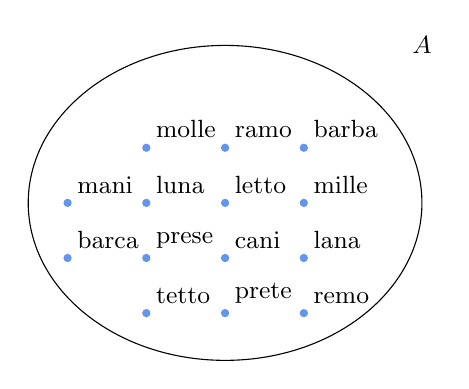
\begin{tikzpicture}[x=10mm,y=10mm, font=\small]
\draw (0,0) circle [x radius=2.5, y radius=2];

\node  at (2.5,2) {$A$};
 \begin{scope}[fill=CornflowerBlue]
\fill (0,0) circle (1.5pt) node[above right] {letto};
\fill (-1,0) circle (1.5pt) node[above right] {luna};
\fill (-2,0) circle (1.5pt) node[above right] {mani};
\fill (-2,-.7) circle (1.5pt) node[above right] {barca};
\fill (1,0) circle (1.5pt) node[above right] {mille};
\fill (0,.7) circle (1.5pt) node[above right] {ramo};
\fill (1,.7) circle (1.5pt) node[above right] {barba};
\fill (-1,.7) circle (1.5pt) node[above right] {molle};
\fill (0,-.7) circle (1.5pt) node[above right] {cani};
\fill (1,-.7) circle (1.5pt) node[above right] {lana};
\fill (-1,-.7) circle (1.5pt) node[above right] {prese}; 
\fill (0,-1.4) circle (1.5pt) node[above right] {prete};
\fill (1,-1.4) circle (1.5pt) node[above right] {remo};
\fill (-1,-1.4) circle (1.5pt) node[above right] {tetto}; 
 \end{scope}
\end{tikzpicture}
\end{inaccessibleblock}
\end{center}

\end{esercizio}

\end{multicols}

\begin{esercizio}
\label{ese:B.4}
Nell'insieme~$C = $\{Como, Milano, Venezia, Parma, Brescia, Aosta, Torino, 
Genova, Imperia, Arezzo, Firenze, Grosseto, Napoli, Campobasso, Catanzaro, 
Bologna, Vercelli, Salerno\} è introdotta la relazione~$\Rel$: 
``essere nella stessa regione''. Costruisci l'insieme~$G_\Rel$
\end{esercizio}

\begin{esercizio}
\label{ese:B.5}
Nell'insieme~$S = \{ x / x$ è il nome di un giorno della settimana\} è 
introdotta la relazione~$\Rel$:~$x \in S$, $y \in S$, $x \Rel y$ se e solo 
se ``$x$ ha lo stesso numero di sillabe di~$y$''. Costruisci l'insieme~$G_\Rel$
\end{esercizio}

\begin{esercizio}
\label{ese:B.6}
Nell'insieme~$F = \{ 1, 3, 4, 6, 5, 9, 0, 2 \}$ è introdotta la 
relazione~$\Rel$: ``essere consecutivi''. Costruisci l'insieme~$G_\Rel$
\end{esercizio}
% \end{multicols}

% \begin{inaccessibleblock}[Figura: TODO]
%  \begin{figure}[t]
% \begin{minipage}[b]{.45\textwidth}
%  \centering
%  % (c) 2012 Dimitrios Vrettos - d.vrettos@gmail.com

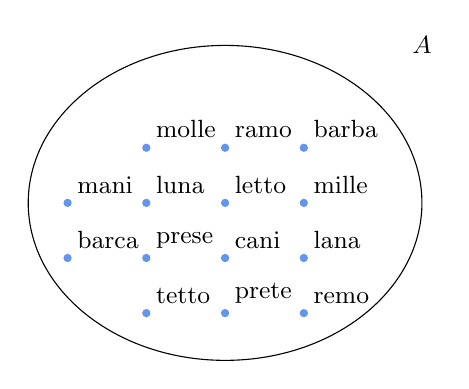
\begin{tikzpicture}[x=10mm,y=10mm, font=\small]
\draw (0,0) circle [x radius=2.5, y radius=2];

\node  at (2.5,2) {$A$};
 \begin{scope}[fill=CornflowerBlue]
\fill (0,0) circle (1.5pt) node[above right] {letto};
\fill (-1,0) circle (1.5pt) node[above right] {luna};
\fill (-2,0) circle (1.5pt) node[above right] {mani};
\fill (-2,-.7) circle (1.5pt) node[above right] {barca};
\fill (1,0) circle (1.5pt) node[above right] {mille};
\fill (0,.7) circle (1.5pt) node[above right] {ramo};
\fill (1,.7) circle (1.5pt) node[above right] {barba};
\fill (-1,.7) circle (1.5pt) node[above right] {molle};
\fill (0,-.7) circle (1.5pt) node[above right] {cani};
\fill (1,-.7) circle (1.5pt) node[above right] {lana};
\fill (-1,-.7) circle (1.5pt) node[above right] {prese}; 
\fill (0,-1.4) circle (1.5pt) node[above right] {prete};
\fill (1,-1.4) circle (1.5pt) node[above right] {remo};
\fill (-1,-1.4) circle (1.5pt) node[above right] {tetto}; 
 \end{scope}
\end{tikzpicture}
%  \caption{Esercizio \ref{ese:B.3}.}\label{fig:B.11}
% \end{minipage}\hfil
% \begin{minipage}[b]{.45\textwidth}
%  \centering
%  % (c) 2012 Dimitrios Vrettos - d.vrettos@gmail.com
\begin{tikzpicture}[scale=.5, x=7.5mm, y=7.5mm, font=\scriptsize]
\begin{scope}[->]
\draw (0,0) -- (0,7.5);
\draw (0,0) -- (7.5,0);
\end{scope}

\begin{scope}[Maroon, dotted, step=7.5mm]
\draw (0,0) grid (7.5,7.5);
\end{scope}

\foreach \x/\xtext in {1/lunedì,2/martedì}{
\node[below left=.2, rotate=30] at (\x,0) {\xtext};
\node[left=.15] at (0,\x) {\xtext};
}
\begin{scope}[very thick, draw=CornflowerBlue, decoration={crosses, shape size=1.5mm}]
\draw decorate {(1,1) -- (1,1.1)};
\draw decorate {(2,2) -- (2,2.1)};
\end{scope}
\end{tikzpicture}
%  \caption{Esercizio \ref{ese:B.7}.}\label{fig:B.12}
% \end{minipage}
% \end{figure}
% \end{inaccessibleblock}

\begin{comment}
 
%===================================
%\subsubsection*{B.3 - Grafico di una relazione}

\begin{multicols}{2}
\begin{esercizio}
\label{ese:B.7}
Considera l'insieme~$S = \{ x / x$ è il nome di un giorno della settimana\}, 
completa la rappresentazione grafica (figura~\ref{fig:B.12}) 
dell'insieme~$S \times S$, evidenzia poi con una crocetta gli elementi 
dell'insieme~$G_\Rel$ determinato dalla relazione ``$x$ ha lo stesso numero di 
sillabe di~$y$''.
\end{esercizio}

\begin{esercizio}
\label{ese:B.8}
Considera l'insieme~$F =$ \{1, 3, 4, 6, 5, 9, 0, 2\}; fai la rappresentazione 
grafica dell'insieme~$F \times F$ e metti in evidenza con una crocetta gli
elementi dell'insieme~$G_\Rel$ determinato dalla relazione ``essere 
consecutivi''.
\end{esercizio}
\end{multicols}

%\subsubsection*{B.4 - Matrice o tabella di una relazione}

\begin{multicols}{2}
\begin{esercizio}
\label{ese:B.9}
Considera nell'insieme~$A =$ \{$-1$, $+3$, $-7$, $+5$, $-2$, $+4$, $+10$\} 
la relazione~$\Rel$:~$x \in A$, $y \in A$, $x \Rel y$ se e solo se ``$x$
è concorde con~$y$''. Costruiamo una tabella a doppia entrata 
(figura~\ref{fig:B.13})) riportando in orizzontale e in verticale gli elementi 
dell'insieme~$A$
Fissa l'attenzione su una cella e segui le istruzioni:
\begin{itemize*}
\item se~$a \Rel b$ metti~1 nella cella~$(a,b)$
\item altrimenti metti~0 nella cella~$(a,b)$
\end{itemize*}
Prosegui tu seguendo l'esempio.
\end{esercizio}

\osservazione Alla fine tutte le celle sono riempite: compare zero se gli 
elementi della coppia ordinata non sono in relazione, compare~1 al contrario.
La relazione~$\Rel$ è completamente rappresentata.

La tabella costruita si chiama \emph{matrice della relazione}.
Una relazione può sempre essere rappresentata attraverso una matrice.

\begin{esercizio}
\label{ese:B.10}
Nell'insieme~$S = \{ x / x$ è il nome di un giorno della settimana\} è 
introdotta la relazione~$\Rel$:~$x \in S$, $y \in S$, $x \Rel y$
se e solo se ``$x$ ha lo stesso numero di sillabe di~$y$''. 
Rappresenta la relazione con una matrice.
\end{esercizio}

\begin{esercizio}
\label{ese:B.11}
Assegnato il predicato~$\Rel$: ``essere divisibile per'' introdotto 
nell'insieme~$A =\{$ 12, 4, 2, 8, 3, 21, 5, 60~$\}$, rappresenta con una 
matrice la relazione~$\Rel$
\end{esercizio}

\end{multicols}

\begin{inaccessibleblock}[Figura: TODO]
 \begin{figure}[b]
\begin{minipage}[b]{.45\textwidth}
 \centering
 % (c) 2012 Dimitrios Vrettos - d.vrettos@gmail.com

\begin{tikzpicture}[x=10mm,y=10mm, font=\small,table nodes/.style={%
		rectangle,
		draw=black,
 		align=center,
   		minimum height=5mm,
     	text depth=0.5ex,
     	text height=1.5ex,
     	inner xsep=-1pt,
     	outer sep=0pt
	},
	table/.style={%
        matrix of nodes,
        row sep=-\pgflinewidth,
        column sep=-\pgflinewidth,
        nodes={%
            table nodes
        } }]

\matrix (first) [table,text width=7mm,name=table,row 2 column 2/.style=blue,row 5 column 4/.style=blue]
{
{}  & $-1$ & $+3$ & $-7$ & $+5$ & $-2$ & $+4$ & $+10$\\
$-1$ &[blue] 1 &{} &{} &{} &{} &{} &{} \\
$+3$ &{} &{} &{} &{} &{} &{} &{} \\
$-7$ &{} &{} &{} &{} &{} &{} &{} \\
$+5$ &{} &{} &{$0$} &{} &{} &{} &{} \\
$-2$ &{} &{} &{} &{} &{} &{} &{} \\
$+4$ &{} &{} &{} &{} &{} &{} &{} \\
$+10$ &{} &{} &{} &{} &{} &{} &{} \\
};

\end{tikzpicture}
 \caption{Esercizio \ref{ese:B.9}.}\label{fig:B.13}
\end{minipage}\hfil
\begin{minipage}[b]{.45\textwidth}
 \centering
 % (c) 2012 Dimitrios Vrettos - d.vrettos@gmail.com

\begin{tikzpicture}[x=10mm,y=10mm, font=\small, every state/.style={draw=CornflowerBlue}, every loop/.style={draw=Maroon}]
\draw (0,0) circle (2);
\node at (2,2) {$A$};
\node[state]  at (-1.5,0) {};
\node[state] (3) at (-.4,.8) {$+3$};
\node[state]  at (1.1,.5) {};
\node[state]  at (-.5,-.2) {};
\node[state] (10) at (1,-1) {$+10$};
\node[state] (7) at (-.5,-1.2) {$-7$};

\begin{scope}[->]
\path (3) edge[loop above] node{} ()
	(10) edge[loop above] node{} ()
   (7) edge[loop right] node {} ();

\end{scope}
\begin{scope}[-, Maroon]
\draw (10)--(3);
\end{scope}
\end{tikzpicture}
 \caption{Esercizio \ref{ese:B.12}.}\label{fig:B.14}
\end{minipage}
\end{figure}
\end{inaccessibleblock}

% \newpage

%\subsubsection*{B.5 - Grafo di una relazione}

\begin{multicols}{2}
\begin{esercizio}
\label{ese:B.12}
Completa la rappresentazione (figura~\ref{fig:B.14})) con frecce della 
relazione~$\Rel$:~$x \in A$, $y \in A$, $x \Rel y$ se e solo se ``$x$ è 
concorde con~$y$''
nell'insieme~$A =$\{$-1$, $+3$, $-7$, $+5$, $-2$, $+4$, $+10$\}.
% \osservazione Nel completare il disegno dell'esercizio precedente hai dovuto 
% utilizzare una freccia con due punte, infatti le proposizioni
% ``$+3$ è concorde con~$+10$'' e ``$+10$ è concorde con~$+3$'' sono entrambe 
vere. 
% Quando si ha questo caso si può omettere la punta della freccia utilizzando 
% un \emph{arco} che collega gli argomenti del predicato.
\end{esercizio}

\begin{esercizio}
\label{ese:B.13}
Nell'insieme~$A = \{ 1, 2, 3, 4, 5, 6, 7, 8, 9 \}$ è introdotto il 
predicato~$\Rel$: ``essere il doppio``; costruisci l'insieme~$G_\Rel$, 
rappresenta la relazione nei tre modi descritti sopra: con un grafico 
cartesiano, con una matrice, con un grafo.
\end{esercizio}

\begin{esercizio}
\label{ese:B.14}
Sono assegnati i grafi di tre relazioni~$\Rel_1$, $\Rel_2$, $\Rel_3$ 
introdotte in altrettanti insiemi~$A$, $B$, $C$ (figura~\ref{fig:B.15}); 
deduci da essi gli elementi di ciascun insieme e costruisci per ciascuna 
relazione l'insieme~$G_\Rel$
\end{esercizio}

\begin{esercizio}
\label{ese:B.15}
Rappresenta nei tre modi che sono stati descritti (con un grafico cartesiano, 
con una matrice, con un grafo) la relazione~$\Rel$: 
``essere nati nello stesso mese'' introdotta nell'insieme~$C$ degli alunni 
della tua classe.
\end{esercizio}

\begin{esercizio}
\label{ese:B.16}
Nell'insieme~$H = \{ x \in \insN / 21 < x < 40 \}$, $x \Rel y$ se e solo se 
``la somma delle cifre di~$x$ è uguale alla somma delle cifre di~$y$''.
Costruisci~$G_\Rel$ e rappresenta la relazione con una matrice.
\end{esercizio}

\begin{esercizio}
\label{ese:B.17}
Scegli la risposta corretta:
Una relazione $\Rel$ introdotta in un insieme~$A$ determina:
\begin{enumeratea}
 \item un sottoinsieme di~$A$
 \item l'insieme~$A \times A$
 \item un insieme di coppie;
 \item un grafico cartesiano;
 \item un sottoinsieme di~$A \times A$
 \end{enumeratea}
\end{esercizio}

\begin{esercizio}
\label{ese:B.18}
Rappresenta con un grafo la relazione~$\Rel$ rappresentata nel grafico 
cartesiano della figura~\ref{fig:B.16}.
\end{esercizio}
\end{multicols}

\begin{inaccessibleblock}[Figura: TODO]
 \begin{figure}[t]
\begin{minipage}[b]{.69\textwidth}
 \centering
 % (c) 2012 Dimitrios Vrettos - d.vrettos@gmail.com

\begin{tikzpicture}[x=10mm,y=10mm, font=\small, every state/.style={draw=CornflowerBlue, minimum size=0pt}, every loop/.style={draw=Maroon}]
\draw (0,0) circle (1.5);
\node at (1.3,1.5) {$A$};
\node[state] (A) at (-1,0) {$a$};
\node[state] (B) at (.5,.5) {$b$};
\node[state] (C) at (0,-1) {$c$};

\begin{scope}[->]
\path (A) edge[loop above] node{} ()
	(B) edge[loop above] node{} ()
   (C) edge[loop right] node {} ();

\end{scope}
\begin{scope}[->, Maroon]
\draw (A)--(B);
\draw (B)--(C);
\end{scope}

\begin{scope}[xshift=31mm]
\draw (0,0) circle (1.5);
\node at (1.3,1.5) {$B$};
\node[state] (1) at (.8,.6) {$1$};
\node[state] (2) at (1.1,0) {$2$};
\node[state] (3) at (-.5,-.8) {$3$};
\node[state] (4) at (.8,-.8) {$4$};
\node[state] (5) at (-1,0) {$5$};
\node[state] (6) at (-.2,.7) {$6$};

\begin{scope}[->]
\path (6) edge[loop above] node{} ()
	(3) edge[loop left] node {} ();

\end{scope}
\begin{scope}[->, Maroon]
\draw (6)--(1);
\draw (6)--(5);
\draw (4)--(2);
\draw (4)--(3);
\draw (2)--(3);
\end{scope}
\end{scope}

\begin{scope}[xshift=62mm]
\draw (0,0) circle (1.5);
\node at (1.3,1.5) {$C$};
\node[state] (D) at (.9,.6) {$D$};
\node[state] (E) at (.7,-.8) {$E$};
\node[state] (G) at (-.5,-.7) {$G$};
\node[state] (H) at (-.7,0) {$H$};
\node[state] (I) at (-.2,.8) {$I$};

\begin{scope}[->]
\path (I) edge[loop above] node{} ()
	(H) edge[loop left] node {} ()
(G) edge[loop left] node {} ()
(E) edge[loop above] node {} ()
(D) edge[loop below] node {} ();

\end{scope}
\begin{scope}[<->, Maroon]
\draw (D)--(I);
\draw (I)--(H);
\draw (D)--(H);
\draw (G)--(E);
\end{scope}
\end{scope}
\end{tikzpicture}
 \caption{Esercizio \ref{ese:B.14}.}\label{fig:B.15}
\end{minipage}\
\begin{minipage}[b]{.3\textwidth}
 \centering
 % (c) 2012 Dimitrios Vrettos - d.vrettos@gmail.com
\begin{tikzpicture}[ x=7.5mm, y=7.5mm, font=\small]
\begin{scope}[->]
\draw (0,0) -- (0,3.5) node[left] {$y$};
\draw (0,0) -- (3.5,0) node[below] {$x$};
\end{scope}

\begin{scope}[Maroon, dotted, step=7.5mm]
\draw (0,0) grid (3.5,3.5);
\end{scope}

\foreach \x/\xtext in {1/1,2/2,3/3}{
\node[below] at (\x,0) {\xtext};
\node[left] at (0,\x) {\xtext};
}
\foreach \x in {1,2,3}{
\draw (\x,1.5pt) -- (\x,-1.5pt);
\draw (1.5pt,\x) -- (-1.5pt,\x);}
\node[below left] at (0,0) {0};
\begin{scope}[very thick, draw=CornflowerBlue, decoration={crosses, shape size=1.5mm}]
\draw decorate {(1,1) -- (1,1.1)};
\draw decorate {(2,2) -- (2,2.1)};
\draw decorate {(1,3) -- (1,3.1)};
\draw decorate {(2,1) -- (2,1.1)};
\draw decorate {(3,2) -- (3,2.1)};
\draw decorate {(3,3) -- (3,3.1)};
\end{scope}
\end{tikzpicture}
 \caption{Esercizio \ref{ese:B.18}.}\label{fig:B.16}
\end{minipage}
\end{figure}
\end{inaccessibleblock}

% \newpage

\end{comment}

% Modificato da Daniele Zambelli: non più:
%\subsubsection*{B.6 - Proprietà riflessiva}  
% ma solo:
%\subsubsection*{\numnameref{sec:B_proprieta}}

% \newpage %---------------------------------------------------

\begin{esercizio}
\label{ese:B.19}
Quali relazioni sono riflessive?
\begin{center}
\begin{tabular}{llc}
\toprule
Insieme & Relazione & È riflessiva?\\
\midrule
Numeri naturali & essere divisibile per &  \boxSi\quad\boxNo \\
% Libri che hai in cartella & avere lo stesso numero di pagine & 
%  \boxSi\quad\boxNo \\
Rette del piano & essere perpendicolare a &  \boxSi\quad\boxNo \\
Rette del piano & essere parallela a &  \boxSi\quad\boxNo \\
Poligoni & avere lo stesso numero di lati &  \boxSi\quad\boxNo \\
% Città della Lombardia & terminare con la stessa vocale & 
%  \boxSi\quad\boxNo \\
Parole italiane & essere il plurale di &  \boxSi\quad\boxNo \\
\bottomrule
\end{tabular}
\end{center}
\end{esercizio}

%\subsubsection*{B.7 - Proprietà antiriflessiva}

% \newpage

\begin{esercizio}
\label{ese:B.20}
Quali delle seguenti relazioni sono antiriflessive?
\begin{center}
\begin{tabular}{llc}
\toprule
Insieme & Relazione & È antiriflessiva?\\
\midrule
Numeri naturali & essere multiplo di & \boxSi\quad\boxNo \\
Rette del piano & essere perpendicolare a & \boxSi\quad\boxNo \\
Poligoni & avere lo stesso perimetro & \boxSi\quad\boxNo \\
Città del Piemonte & avere più abitanti di & \boxSi\quad\boxNo \\
Parole italiane & essere il femminile di & \boxSi\quad\boxNo \\
% Fiumi italiani & essere affluente & \boxSi\quad\boxNo \\
% Persone & essere figlio di & \boxSi\quad\boxNo \\
\bottomrule
\end{tabular}
\end{center}
\end{esercizio}

%\subsubsection*{B.8 - Proprietà simmetrica}

\begin{esercizio}
\label{ese:B.21}
Riconosci le relazioni simmetriche:
\begin{center}
\begin{tabular}{llc}
\toprule
Insieme & Relazione & È simmetrica?\\
\midrule
Città d'Italia & appartenere alla stessa regione & \boxSi\quad\boxNo \\
Rette del piano & essere perpendicolari & \boxSi\quad\boxNo \\
Solidi & avere lo stesso volume & \boxSi\quad\boxNo \\
Persone & essere il padre di & \boxSi\quad\boxNo \\
% Persone & essere fratello o sorella di & \boxSi\quad\boxNo \\
% Numeri naturali & avere lo stesso numero di cifre di & \boxSi\quad\boxNo \\
Fiumi d'Europa & essere affluente & \boxSi\quad\boxNo \\
% Numeri interi & essere il quadrato di & \boxSi\quad\boxNo \\
\bottomrule
\end{tabular}
\end{center}

Le relazioni degli ultimi due casi non godono della proprietà simmetrica. 
Infatti:
\begin{itemize} [nosep]
\item la proposizione ``Il Ticino è un affluente del Po'' è vera, ma non lo è 
la proposizione che da essa si ottiene scambiando il soggetto con il 
complemento; \item se un numero intero è il quadrato di un altro 
(ad esempio~$+25$ è il quadrato di~$+5$), non è vero che~$+5$ 
è il quadrato di~$+25$
\end{itemize}
\end{esercizio}

%\subsubsection*{B.9 - Proprietà antisimmetrica}

\begin{esercizio}
\label{ese:B.22}
Riconosci le relazioni antisimmetriche:
\begin{center}
\begin{tabular}{llc}
\toprule
Insieme & Relazione & È antisimmetrica?\\
\midrule
Numeri naturali & essere divisibile per & \boxSi\quad\boxNo \\
Rette del piano & essere perpendicolare a & \boxSi\quad\boxNo \\
Poligoni & avere lo stesso perimetro & \boxSi\quad\boxNo \\
Angoli & essere complementare a & \boxSi\quad\boxNo \\
Città del Lazio & essere nella stessa provincia di & \boxSi\quad\boxNo \\
\bottomrule
\end{tabular}
\end{center}
\end{esercizio}

%\subsubsection*{B.10 - Proprietà transitiva}

\begin{comment}
 ???????????????????
\begin{enumeratea}
\item da~$18 \Rel~50$ e~$50 \Rel \ldots$ segue~$\ldots \Rel \ldots$
\item da~$\ldots \Rel~555$ e~$\ldots \Rel~267$ segue~$\ldots \Rel \ldots$
\end{enumeratea}
\end{esercizio}

\begin{esercizio}
\label{ese:B.23}
Verifica se, nell'insieme ~$\insN$ dei numeri naturali, la relazione~$\Rel$: 
``avere lo stesso numero di cifre'' gode della proprietà transitiva.
Completa le proposizioni e rappresenta~$\Rel$ con un grafo:

% \newpage

\begin{esercizio}
\label{ese:B.24}
Indica quale tra le seguenti relazioni è transitiva:
\begin{center}
\begin{tabular}{llc}
\toprule
Insieme & Relazione & È transitiva?\\
\midrule
Numeri naturali & essere multiplo di & \boxSi\quad\boxNo \\
Regioni d'Italia & essere più a nord di & \boxSi\quad\boxNo \\
Numeri interi & essere minore di & \boxSi\quad\boxNo \\
Rette del piano & essere perpendicolari & \boxSi\quad\boxNo \\
Persone & essere padre di & \boxSi\quad\boxNo \\
Stati d'Europa & confinare con & \boxSi\quad\boxNo \\
\bottomrule
\end{tabular}
\end{center}
\end{esercizio}

\begin{esercizio}
\label{ese:B.25}
Dai una rappresentazione tabulare 
dell'insieme~$H = \{ x \in \insN / 0 \leq x \leq~12 \}$ 
determina il resto della divisione di ciascun numero di~$H$ con~4,
compila la tabella come suggerito nell'esempio:
\begin{center}
\begin{tabular}{lccccccccccccc}
\toprule
operazione & $0:4$ & $1:4$ & $2:4$ & & & & & & & & & & $12:4$ \\
resto & 0 & 1 & & & & & & & & & & & 0 \\
\bottomrule
\end{tabular}
\end{center}
Introduciamo in~$H$ la relazione~$x \Rel y$ se e solo se ``$x$ e~$y$ hanno lo 
stesso resto nella divisione per~4''.
Costruisci il grafo della relazione e stabilisci se gode della proprietà 
transitiva.

La stessa relazione~$\Rel$ introdotta nell'insieme dei numeri naturali~$\insN$ 
è una relazione transitiva?
\end{esercizio}

\begin{multicols}{2}
\begin{esercizio}
\label{ese:B.26}
Completa il grafo (figura~\ref{fig:B.17}) in modo che la relazione 
rappresentata diventi transitiva.
\end{esercizio}

\begin{esercizio}
\label{ese:B.27}
Indica la risposta corretta:

\begin{enumeratea}
\TabPositions{12cm}
\item se una relazione è simmetrica, all'insieme~$G_\Rel$ appartengono le 
coppie del tipo~$(a,b)$ e~$(b,a)$
\item il grafico cartesiano è un modo per rappresentare una relazione;
\item la matrice di una relazione riflessiva presenta tutti uno sulla 
 diagonale discendente;
\item la matrice di una relazione antiriflessiva non presenta alcun uno sulla 
 diagonale discendente;
\item se una relazione è transitiva, allora è anche simmetrica;
\item se~$(x,y) \in G_\Rel$ e~$(y,z) \in G_\Rel$ qualche volta si 
 ha~$(x,z) \in G_\Rel$
\item se~$(x,y) \in G_\Rel$ si ha sempre~$(y,x) \in G_\Rel$
\item una relazione riflessiva presenta nel suo grafo il cappio su ciascun 
 elemento;
\item una relazione binaria è individuata da un predicato che lega due 
 argomenti dell'insieme~$A$
\item una relazione binaria genera un sottoinsieme del prodotto 
 cartesiano~$A \times~A$
\end{enumeratea}
\end{esercizio}

\begin{esercizio}
\label{ese:B.28}
Con riferimento al grafico cartesiano disegnato nella figura~\ref{fig:B.18}, 
quale è vera?

\begin{enumeratea}
\item nel suo grafo almeno un elemento non presenta il cappio;
\item la relazione è antisimmetrica;
\item la relazione è transitiva;
\item l'insieme~$G_\Rel$ è costituito dalle 
coppie~$(1,2)$, $(1,4)$, $(3,4)$, $(4,2)$
\end{enumeratea}
\end{esercizio}
\end{multicols}
\begin{inaccessibleblock}[Figura: TODO]
 \begin{figure}[t]
\begin{minipage}[b]{.45\textwidth}
 \centering
 % (c) 2012 Dimitrios Vrettos - d.vrettos@gmail.com

\begin{tikzpicture}[x=10mm,y=10mm, font=\small, every state/.style={draw=CornflowerBlue, minimum size=0pt}]

\node[state] (X) at (-1,0) {$X$};
\node[state] (H) at (.5,.5) {$H$};
\node[state] (K) at (1,-1) {$K$};
\node[state] (Z) at (-.5,-1) {$Z$};

\begin{scope}[->, Maroon]
\draw (X)--(H);
\draw (X)--(Z);
\draw (H)--(K);
\end{scope}

\end{tikzpicture}

 \caption{Esercizio \ref{ese:B.26}.}\label{fig:B.17}
\end{minipage}\
\begin{minipage}[b]{.45\textwidth}
 \centering
 % (c) 2012 Dimitrios Vrettos - d.vrettos@gmail.com
\begin{tikzpicture}[ x=7.5mm, y=7.5mm, font=\small]
\begin{scope}[->]
\draw (0,0) -- (0,4.5) node[left] {$y$};
\draw (0,0) -- (4.5,0) node[below] {$x$};
\end{scope}

\begin{scope}[Maroon, dotted, step=7.5mm]
\draw (0,0) grid (4.5,4.5);
\end{scope}

\foreach \x/\xtext in {1/1,2/2,3/3,4/4}{
\node[below] at (\x,0) {\xtext};
\node[left] at (0,\x) {\xtext};
}
\foreach \x in {1,2,3,4}{
\draw (\x,1.5pt) -- (\x,-1.5pt);
\draw (1.5pt,\x) -- (-1.5pt,\x);}
\node[below left] at (0,0) {0};
\begin{scope}[very thick, draw=CornflowerBlue, decoration={crosses, shape size=1.5mm}]
\draw decorate {(1,2) -- (1,2.1)};
\draw decorate {(1,4) -- (1,4.1)};
\draw decorate {(3,4) -- (3,4.1)};
\draw decorate {(4,2) -- (4,2.1)};
\end{scope}
\end{tikzpicture}
 \caption{Esercizio \ref{ese:B.28}.}\label{fig:B.18}
\end{minipage}
\end{figure}
\end{inaccessibleblock}

% \newpage

\end{comment}

\newpage %---------------------------------------------------

\begin{esercizio}
\label{ese:B.29}
Quali proprietà verificano le seguenti relazioni?
\begin{center}
R = riflessiva; AR = antiriflessiva; S = simmetrica; AS = antisimmetrica; 
T = transitiva
\end{center}
\begin{center}
\begin{tabular}{llc}
\toprule
Insieme & Relazione & Proprietà\\
\midrule
Poligoni del piano & avere lo stesso numero di lati & 
 \boxR\quad\boxAR\quad\boxS\quad\boxAS\quad\boxT\\
Numeri naturali & avere lo stesso numero di cifre &
 \boxR\quad\boxAR\quad\boxS\quad\boxAS\quad\boxT\\
Numeri naturali & essere minore di &
 \boxR\quad\boxAR\quad\boxS\quad\boxAS\quad\boxT\\
Numeri naturali & essere divisibile per &
 \boxR\quad\boxAR\quad\boxS\quad\boxAS\quad\boxT\\
$A = \{ x \in \insN / 1 \leq x \leq~5 \}$ & essere multiplo di &
 \boxR\quad\boxAR\quad\boxS\quad\boxAS\quad\boxT\\
\bottomrule
\end{tabular}
\end{center}
\end{esercizio}

% \newpage

%\subsubsection*{B.11 - Relazioni di equivalenza}
% \subsubsection*{\numnameref{subsec:rel_equivalenza}}

\begin{esercizio}
\label{ese:B.30}
Quali delle seguenti sono relazioni di equivalenza?
\begin{center}
\begin{tabular}{llc}
\toprule
Relazione & Insieme & È d'equivalenza?\\
\midrule
Essere multiplo & numeri naturali & \boxV\quad\boxF \\
Avere lo stesso numero di sillabe & parole italiane & \boxV\quad\boxF\\
Essere minore & interi relativi & \boxV\quad\boxF \\
Vincere & squadre di calcio & \boxV\quad\boxF\\
Avere lo stesso numero di angoli & poligoni & \boxV\quad\boxF \\
% Essere il plurale & parole italiane & \boxV\quad\boxF \\
% Essere il cubo & numeri interi & \boxV\quad\boxF \\
\bottomrule
\end{tabular}
\end{center}
\end{esercizio}

% \begin{inaccessibleblock}[Figura: TODO]
%  \begin{figure}[t]
%  \centering% (c) 2012 Dimitrios Vrettos - d.vrettos@gmail.com

\begin{tikzpicture}[x=10mm,y=10mm, font=\small, every state/.style={draw=CornflowerBlue, minimum size=0pt}, every loop/.style={draw=Maroon}]
\draw (0,0) circle (1.5);
\node at (1.3,1.5) {$A$};
\node at (0,-2) {caso 1};
\node[state] (1) at (-1,0) {$a$};
\node[state] (2) at (.5,.7) {$b$};
\node[state] (3) at (1,0) {$c$};
\node[state] (4) at (-.6,-.7) {$d$};
\node[state] (5) at (.5,-.5) {$e$};
\node[state] (6) at (-.2,.2) {$f$};
\node[state] (7) at (.2,-1.1) {$g$};
\node[state] (8) at (-.4,1.1) {$h$};
\begin{scope}[->]
\path (1) edge[loop above] node{} ()
	(2) edge[loop above] node{} ()
   (6) edge[loop below] node {} ()
(3) edge[loop above] node{} ()
(4) edge[loop left] node{} ()
(7) edge[loop right] node{} ();

\end{scope}
\begin{scope}[-, Maroon]
\draw (1)--(8);
\draw (1)--(6);
\draw (8)--(6);

\draw (2)--(3);
\draw (2)--(5);
\draw (3)--(5);

\draw (4)--(7);
\end{scope}

 \begin{scope}[xshift=32mm]
\draw (0,0) circle (1.5);
\node at (1.3,1.5) {$B$};
\node at (0,-2) {caso 2};
\node[state] (1) at (-1,0) {$a$};
\node[state] (2) at (.5,.7) {$b$};
\node[state] (3) at (1,0) {$c$};
\node[state] (4) at (-.6,-.7) {$d$};
\node[state] (5) at (.5,-.5) {$e$};
\node[state] (6) at (-.2,.2) {$f$};
\node[state] (7) at (.2,-1.1) {$g$};
\node[state] (8) at (-.4,1.1) {$h$};
\begin{scope}[->]
\path (1) edge[loop above] node{} ()
	(2) edge[loop above] node{} ()
   (6) edge[loop below] node {} ()
(3) edge[loop above] node{} ()
(4) edge[loop left] node{} ()
(7) edge[loop right] node{} ()
(5) edge[loop right] node{} ()
(8) edge[loop right] node{} ();

\end{scope}
\begin{scope}[-, Maroon]
\draw (1)--(8);
\draw (1)--(6);
\draw (8)--(6);

\draw (2)--(3);
\draw (2)--(5);
\draw (3)--(5);

\draw (4)--(7);
\end{scope}
 \end{scope}

 \begin{scope}[xshift=64mm]
\draw (0,0) circle (1.5);
\node at (1.3,1.5) {$C$};
\node at (0,-2) {caso 3};
\node[state] (1) at (-1,0) {$a$};
\node[state] (2) at (.5,.7) {$b$};
\node[state] (3) at (1,0) {$c$};
\node[state] (4) at (-.6,-.7) {$d$};
\node[state] (5) at (.5,-.5) {$e$};

\begin{scope}[->]
\path (1) edge[loop above] node{} ()
	(2) edge[loop above] node{} ()
(3) edge[loop above] node{} ()
(4) edge[loop left] node{} ()
(5) edge[loop right] node{} ();

\end{scope}
\begin{scope}[-, Maroon]
\draw (1)--(2);
\draw (2)--(3);
\draw (4)--(5);
\end{scope}
 \end{scope}

 \begin{scope}[xshift=96mm]
\draw (0,0) circle (1.5);
\node at (1.3,1.5) {$D$};
\node at (0,-2) {caso 4};
\node[state] (1) at (-1,0) {$a$};
\node[state] (2) at (.5,.7) {$b$};
\node[state] (3) at (1,0) {$c$};
\node[state] (4) at (-.6,-.7) {$d$};
\node[state] (6) at (.5,-.5) {$f$};
\begin{scope}[->]
\path (1) edge[loop above] node{} ()
	(2) edge[loop above] node{} ()
   (6) edge[loop below] node {} ()
(3) edge[loop above] node{} ()
(4) edge[loop left] node{} ();

\end{scope}
\begin{scope}[->, Maroon]
\draw (3)--(1);
\draw (2)--(1);
\draw (2)--(3);
\end{scope}
 \end{scope}
\end{tikzpicture}
%  \caption{Esercizio \ref{ese:B.31}}\label{fig:B.19}
% \end{figure}
% \end{inaccessibleblock}

\begin{esercizio}
\label{ese:B.31}
Analizza i grafi nella figura e individua quello che 
rappresenta una relazione d'equivalenza.

\begin{center}
\begin{inaccessibleblock}[Figura: TODO]
 % (c) 2012 Dimitrios Vrettos - d.vrettos@gmail.com

\begin{tikzpicture}[x=10mm,y=10mm, font=\small, every state/.style={draw=CornflowerBlue, minimum size=0pt}, every loop/.style={draw=Maroon}]
\draw (0,0) circle (1.5);
\node at (1.3,1.5) {$A$};
\node at (0,-2) {caso 1};
\node[state] (1) at (-1,0) {$a$};
\node[state] (2) at (.5,.7) {$b$};
\node[state] (3) at (1,0) {$c$};
\node[state] (4) at (-.6,-.7) {$d$};
\node[state] (5) at (.5,-.5) {$e$};
\node[state] (6) at (-.2,.2) {$f$};
\node[state] (7) at (.2,-1.1) {$g$};
\node[state] (8) at (-.4,1.1) {$h$};
\begin{scope}[->]
\path (1) edge[loop above] node{} ()
	(2) edge[loop above] node{} ()
   (6) edge[loop below] node {} ()
(3) edge[loop above] node{} ()
(4) edge[loop left] node{} ()
(7) edge[loop right] node{} ();

\end{scope}
\begin{scope}[-, Maroon]
\draw (1)--(8);
\draw (1)--(6);
\draw (8)--(6);

\draw (2)--(3);
\draw (2)--(5);
\draw (3)--(5);

\draw (4)--(7);
\end{scope}

 \begin{scope}[xshift=32mm]
\draw (0,0) circle (1.5);
\node at (1.3,1.5) {$B$};
\node at (0,-2) {caso 2};
\node[state] (1) at (-1,0) {$a$};
\node[state] (2) at (.5,.7) {$b$};
\node[state] (3) at (1,0) {$c$};
\node[state] (4) at (-.6,-.7) {$d$};
\node[state] (5) at (.5,-.5) {$e$};
\node[state] (6) at (-.2,.2) {$f$};
\node[state] (7) at (.2,-1.1) {$g$};
\node[state] (8) at (-.4,1.1) {$h$};
\begin{scope}[->]
\path (1) edge[loop above] node{} ()
	(2) edge[loop above] node{} ()
   (6) edge[loop below] node {} ()
(3) edge[loop above] node{} ()
(4) edge[loop left] node{} ()
(7) edge[loop right] node{} ()
(5) edge[loop right] node{} ()
(8) edge[loop right] node{} ();

\end{scope}
\begin{scope}[-, Maroon]
\draw (1)--(8);
\draw (1)--(6);
\draw (8)--(6);

\draw (2)--(3);
\draw (2)--(5);
\draw (3)--(5);

\draw (4)--(7);
\end{scope}
 \end{scope}

 \begin{scope}[xshift=64mm]
\draw (0,0) circle (1.5);
\node at (1.3,1.5) {$C$};
\node at (0,-2) {caso 3};
\node[state] (1) at (-1,0) {$a$};
\node[state] (2) at (.5,.7) {$b$};
\node[state] (3) at (1,0) {$c$};
\node[state] (4) at (-.6,-.7) {$d$};
\node[state] (5) at (.5,-.5) {$e$};

\begin{scope}[->]
\path (1) edge[loop above] node{} ()
	(2) edge[loop above] node{} ()
(3) edge[loop above] node{} ()
(4) edge[loop left] node{} ()
(5) edge[loop right] node{} ();

\end{scope}
\begin{scope}[-, Maroon]
\draw (1)--(2);
\draw (2)--(3);
\draw (4)--(5);
\end{scope}
 \end{scope}

 \begin{scope}[xshift=96mm]
\draw (0,0) circle (1.5);
\node at (1.3,1.5) {$D$};
\node at (0,-2) {caso 4};
\node[state] (1) at (-1,0) {$a$};
\node[state] (2) at (.5,.7) {$b$};
\node[state] (3) at (1,0) {$c$};
\node[state] (4) at (-.6,-.7) {$d$};
\node[state] (6) at (.5,-.5) {$f$};
\begin{scope}[->]
\path (1) edge[loop above] node{} ()
	(2) edge[loop above] node{} ()
   (6) edge[loop below] node {} ()
(3) edge[loop above] node{} ()
(4) edge[loop left] node{} ();

\end{scope}
\begin{scope}[->, Maroon]
\draw (3)--(1);
\draw (2)--(1);
\draw (2)--(3);
\end{scope}
 \end{scope}
\end{tikzpicture}
\end{inaccessibleblock}
\end{center}

\begin{description} [nosep]
\item [caso~1] non è rappresentata una relazione d'equivalenza perché 
 \dotfill
\item [caso~2] la presenza del cappio su ciascun elemento indica che la 
relazione gode della proprietà \ldots,
il fatto che coppie di elementi siano collegate da archi indica che vale la 
proprietà \ldots, infine terne di elementi godono della proprietà \dotfill

In conclusione \dotfill
\item [caso~3] non gode della proprietà \dotfill, 
pertanto \dotfill
\item [caso~4] sussistono le proprietà \ldots e \ldots, ma non la proprietà 
\ldots pertanto la relazione \dotfill
\end{description}
\end{esercizio}

\begin{comment}

\begin{multicols}{2}
\begin{esercizio}
\label{ese:B.32}
Fissa l'attenzione sulla relazione~$\Rel$: ``frequentare la stessa classe'' 
introdotta nell'insieme~$S$ degli alunni iscritti nella tua scuola.
Verifica che~$\Rel$ è una relazione d'equivalenza. Costruisci le classi 
d'equivalenza. Quante ne hai potuto formare? Come sono indicate nella
realtà che vivi quotidianamente? Determina la partizione~$P(S)$ in classi 
d'equivalenza e infine l'insieme quoziente~$S/\Rel$
\end{esercizio}

\begin{esercizio}
\label{ese:B.33}
Studia in~$\insN$ la relazione~$\Rel$: ``avere la stessa cifra delle unità''. 
Verifica se è una relazione d'equivalenza, costruisci l'insieme quoziente 
dopo aver risposto alle seguenti domande:\vspace{-1ex}
\begin{itemize*}
\item quanti numeri naturali sono tra loro equivalenti?
\item da quanti elementi è costituito l'insieme~$\insN/\Rel$?
\item qual è l'elemento che sceglieresti come rappresentante di ciascuna 
 classe?
\end{itemize*}
\end{esercizio}

\begin{esercizio}
\label{ese:B.34}
Considera la relazione~$\Rel$: 
``avere lo stesso resto nella divisione per due'' 
introdotta nell'insieme~$\insN$ e studiane le proprietà.
\begin{itemize*}
\item è una relazione d'equivalenza? Se la risposta è affermativa, costruisci 
 l'insieme quoziente~$\insN/\Rel$
\item quante classi d'equivalenza hai formato?
\item puoi sfruttare quanto ottenuto per enunciare le definizioni di numero 
 pari e di numero dispari?
\item giustifica, in base allo svolgimento dell'esercizio, l'affermazione: 
``L'insieme dei numeri pari è il complementare in~$\insN$ dell'insieme dei 
numeri dispari''.
\end{itemize*}
\end{esercizio}

\begin{esercizio}
\label{ese:B.35}
Considera l'insieme~$A = \{ x \in \insN / 1 \leq x \leq~20 \}$ e i suoi
sottoinsiemi:~$A_1 =$\{1, 5, 9, 13, 17\}; $A_2 =$\{ 2, 6, 10, 14, 18 \}; 
$A_3 =$\{ 3, 7, 11, 15, 19 \}; $A_4 =$\{ 4, 8, 12, 16, 20 \}.
\begin{enumeratea}
\item Rappresenta gli insiemi con un diagramma di Eulero-Venn;
\item si può affermare che quei sottoinsiemi determinano una partizione 
 dell'insieme~$A$?
\item è vero che a ciascuno dei suddetti sottoinsiemi appartengono i numeri 
 di~$A$ aventi lo stesso resto nella divisione per~4?
\item quei sottoinsiemi sono dunque classi d'equivalenza? 
 Qual è il predicato della relazione che le determina?
\end{enumeratea}
\end{esercizio}

\begin{esercizio}
\label{ese:B.36}
Nell'insieme ~$\insN$ dei numeri naturali stabilisci se è d'equivalenza la 
relazione~$\Rel$: ``$x \Rel y$ se e solo se~$x$ ha le stesse cifre di~$y$''.
\end{esercizio}

\begin{esercizio}
\label{ese:B.37}
Nell'insieme~$C$ degli alunni della tua classe verifica se la 
relazione~$\Rel$: ``$x \Rel y$ se e solo se il cognome di~$x$ ha la stessa 
lettera iniziale del cognome di~$y$'' è d'equivalenza; determina in caso 
affermativo la partizione dell'insieme~$C$ e l'insieme quoziente~$C/\Rel$
\end{esercizio}

% \begin{esercizio}
% \label{ese:B.38}
% Nell'insieme delle parole della lingua italiana verifica se la relazione 
% ``$x \Rel y$ se e solo se~$x$ ha lo stesso numero di lettere di~$y$'' è
% una relazione di equivalenza. In caso affermativo individua alcune classi di
% equivalenza.
% \end{esercizio}

\begin{esercizio}
\label{ese:B.39}
Nell'insieme dei nomi dei giorni della settimana considera la relazione 
``$x \Rel y$ se e solo se~$x$ e~$y$ hanno almeno tre lettere in comune''.
Verifica se è una relazione di equivalenza e in caso affermativo individua le
classi di equivalenza.
\end{esercizio}

\begin{esercizio}
\label{ese:B.40}
Nell'insieme dei numeri naturali da~1 a~100, verifica se la relazione 
``$x \Rel y$ se e solo se~$x$ e~$y$ hanno lo stesso numero di lettere''
è una relazione di equivalenza. Individua quante sono le classi di equivalenza.
Scrivi tutti gli elementi delle classi di equivalenza~$[1]$ e~$[10]$
\end{esercizio}

\begin{esercizio}
\label{ese:B.41}
Nell'insieme dei numeri naturali da~1 a~100, verifica se la relazione 
``$x \Rel y$ se e solo se~$x+y$ è dispari'' è una relazione di equivalenza.
\end{esercizio}

\begin{esercizio}
\label{ese:B.42}
Nell'insieme dei nomi dei mesi dell'anno verifica se la relazione ``$x \Rel y$ 
se e solo se~$x$ e~$y$ hanno almeno~3 lettere in comune'' è una relazione di 
equivalenza. Eventualmente individua le classi di equivalenza.
\end{esercizio}

\begin{esercizio}
\label{ese:B.43}
Sia~$S$ un insieme non vuoto in cui è definita una relazione~$\Rel$ riflessiva 
e transitiva; in~$S$ si definisca la relazione~$\sharp$ ponendo,
per ogni~$x$, $y$ appartenenti a~$X$, $x \sharp y$ 
se e solo se~$x \Rel y$ e~$y \Rel x$ Verificare che~$\sharp$ è relazione di 
equivalenza in~$X$
\end{esercizio}
\end{multicols}

\begin{inaccessibleblock}[Figura: TODO]
 \begin{figure}[t]
\begin{minipage}[b]{.45\textwidth}
 \centering
 % (c) 2012 Dimitrios Vrettos - d.vrettos@gmail.com

\begin{tikzpicture}[x=10mm,y=10mm, font=\small, every state/.style={draw=CornflowerBlue, minimum size=0pt}, every loop/.style={draw=Maroon}]
\draw (0,0) circle (1.5);
\node at (1.5,1.5) {$T$};
\node[state] (1) at (-.6,.7) {$M$};
\node[state] (2) at (1,.5) {$Z$};
\node[state] (3) at (1,-.5) {$W$};
\node[state] (4) at (-.8,-.7) {$J$};
\node[state] (5) at (0.1,-1.1) {$P$};

\begin{scope}[->, Maroon]
 \draw (1)--(3);
 \draw (1)--(2);
 \draw (2)--(3); 
 \draw (2)--(5); 
 \draw (2)--(4); 
 \draw (3)--(4);
 \draw (5)--(4);
 \draw (5)--(3);
 \draw (1)--(4);
 \draw (1)--(5);
\end{scope}

\end{tikzpicture}

 \caption{Esercizio \ref{ese:B.45}.}\label{fig:B.20}
\end{minipage}\
\begin{minipage}[b]{.45\textwidth}
 \centering
 % (c) 2012 Dimitrios Vrettos - d.vrettos@gmail.com
\begin{tikzpicture}[ x=7.5mm, y=7.5mm, font=\small]
\begin{scope}[->]
\draw (0,0) -- (0,4.5) node[left] {$y$};
\draw (0,0) -- (4.5,0) node[below] {$x$};
\end{scope}

\begin{scope}[Maroon, dotted, step=7.5mm]
\draw (0,0) grid (4.5,4.5);
\end{scope}

\foreach \x/\xtext in {1/5,2/7,3/10,4/20}{
\node[below] at (\x,0) {\xtext};
\node[left] at (0,\x) {\xtext};
}
\foreach \x in {1,2,3,4}{
\draw (\x,1.5pt) -- (\x,-1.5pt);
\draw (1.5pt,\x) -- (-1.5pt,\x);}
\node[below left] at (0,0) {0};
\begin{scope}[very thick, draw=CornflowerBlue, decoration={crosses, shape size=1.5mm}]
\draw decorate {(1,1) -- (1,1.1)};
\draw decorate {(1,2) -- (1,2.1)};
\draw decorate {(1,3) -- (1,3.1)};
\draw decorate {(1,4) -- (1,4.1)};
\draw decorate {(2,3) -- (2,3.1)};
\draw decorate {(2,4) -- (2,4.1)};
\draw decorate {(4,3) -- (4,3.1)};
\draw decorate {(4,4) -- (4,4.1)};
\end{scope}
\end{tikzpicture}
 \caption{Esercizio \ref{ese:B.47}.}\label{fig:B.21}
\end{minipage}
\end{figure}
\end{inaccessibleblock}

%\subsubsection*{B.12 - Relazioni di ordine}
% \subsubsection*{\numnameref{sec:B_ordine}}

\begin{multicols}{2}
\begin{esercizio}
\label{ese:B.44}
Nell'insieme~$M =$\{1, 8, 3, 4, 10, 2, 7, 0, 5, 9, 6\} viene introdotta la 
relazione~$\Rel$ così definita: ``$x \Rel y$ se e solo se~$y-x$ appartiene 
a~$\insN$''.
La relazione è riflessiva? La relazione è antisimmetrica? La relazione è 
transitiva? È vero che due elementi distinti sono sempre confrontabili?
\end{esercizio}

\begin{esercizio}
\label{ese:B.45}
È assegnata la relazione~$R$ nell'insieme~$T$, rappresentata col grafo 
(figura~\ref{fig:B.20}).
Analizzando il grafo, rispondi alle domande:
\begin{itemize*}
\item la relazione è riflessiva?
\item la relazione è antisimmetrica?
\item la relazione è transitiva?
\item due elementi distinti sono sempre confrontabili?
\end{itemize*}
Alla prima domanda avrai risposto negativamente: nessun elemento 
dell'insieme~$T$ è in relazione con se stesso, mentre valgono le proprietà 
antisimmetrica e transitiva.
Infine scelti due elementi qualsiasi dell'insieme~$T$, essi sono sempre 
confrontabili.
\end{esercizio}

\begin{esercizio}
\label{ese:B.46}
Verifica che la relazione~$\Rel$: ``essere divisore'' introdotta 
nell'insieme~$J =$\{3, 6, 10, 15, 21\} è una relazione d'ordine parziale in 
senso largo.
\end{esercizio}

\begin{esercizio}
\label{ese:B.47}
Perché la relazione~$\Rel$ assegnata con il grafico cartesiano riportato 
nella figura~\ref{fig:B.21}, pur essendo una relazione d'ordine non può essere
classificata in nessuna delle tipologie studiate? Dai una breve motivazione 
indicando quali proprietà non sono soddisfatte dalla relazione rappresentata.

\end{esercizio}

\end{comment}

\begin{esercizio}
\label{ese:B.48}
Nell'insieme degli studenti della tua classe determina le proprietà della 
relazione~$\Rel$: ``$x \Rel y$ se e solo se l'altezza di~$x$ non supera 
l'altezza di~$y$''. È una relazione d'ordine? Di quale tipo?
\end{esercizio}

\begin{esercizio}
\label{ese:B.49}
Nell'insieme~$A = \{ 12, 4, 2, 8, 3, 21, 5, 60 \}$ la relazione~$\Rel$: 
``essere divisibile'' è una relazione d'ordine? Se lo è di che tipo di 
relazione si tratta? Totale, parziale, in senso largo, in senso stretto.
\end{esercizio}

\begin{esercizio}
\label{ese:B.50}
Nell'insieme ~$\insN - \{ 0 \}$ la relazione ``essere divisibile'' è d'ordine 
totale in senso largo?
\end{esercizio}

\begin{esercizio}
\label{ese:B.53}
La relazione~$\Rel$: ``essere vicini di banco'' inserita nell'insieme degli 
alunni della tua classe è una relazione d'equivalenza? 
È una relazione d'ordine?
\end{esercizio}

\begin{esercizio}
\label{ese:B.55}
Nell'insieme ~$\insN$ la relazione~$\Rel$: 
''$x \Rel y$ se e solo se~$x \cdot y$ è un numero dispari'' è d'equivalenza?
\end{esercizio}

\begin{esercizio}
\label{ese:B.57}
Verifica se la relazione~$\Rel$ assegnata con la matrice rappresentata
sotto è d'equivalenza, in caso positivo determina la partizione 
dell'insieme~$A =\{\square, \lozenge, \infty, \nabla\}$ e l'insieme
quoziente~$A/\Rel$
\end{esercizio}

\begin{comment}

\begin{esercizio}
\label{ese:B.51}
Rappresenta nelle tre modalità studiate una relazione che sia solo simmetrica; 
ripeti le rappresentazioni per una relazione che sia almeno simmetrica. 
Quale significato hanno le due richieste formulate sopra?
\end{esercizio}

\begin{esercizio}
\label{ese:B.52}
L'insieme~$G_\Rel$ di una relazione introdotta 
nell'insieme~$A = \{ a, b, c, d, e \}$ 
è~$G_\Rel =$ \{ $(a,a)$ $(a,b)$ $(b,b)$ $(d,d)$ $(c,d)$ $(d,e)$ $(e,e)$\}.
Quale delle seguenti affermazioni è vera
\begin{enumeratea}
\item $\Rel$ è una relazione antiriflessiva
\item $\Rel$ è una relazione solo antisimmetrica
\item $\Rel$ è una relazione riflessiva
\item $\Rel$ è una relazione transitiva e antisimmetrica
\end{enumeratea}
\end{esercizio}


\begin{esercizio}
\label{ese:B.54}
I tre sottoinsiemi~$A_1 = \{ 36, 135, 432 \}$ 
$A_2 = \{ 65 \}$ $A_3 = \{ 66, 3522, 93, 435 \}$
dell'insieme~$A = \{ 36, 65, 66, 93, 135, 432, 435, 3522 \}$ 
costituiscono una partizione dell'insieme~$A$? Sapresti trovare una 
caratteristica per gli elementi di ciascun sottoinsieme? 
$A_1$, $A_2$, $A_3$ sono classi d'equivalenza?
\end{esercizio}

\begin{esercizio}
\label{ese:B.56}
La relazione~$\Rel$: 
''$x \Rel y$ se e solo se~$x$ sta nella stessa nazione di~$y$'' 
nell'insieme~$K=$ \{Parigi, Madrid, Milano, Siviglia, Bari, Granata, 
Venezia, Lione\}
è d'equivalenza? Costruisci~$A/\Rel$
\end{esercizio}

\begin{center}
\begin{tabular}{ccccc}
\toprule
 & $\square$ & $\lozenge$ & $\infty$ & $\nabla$\\
\midrule
 $\square$ & 1 & 1 & 0 & 0 \\
 $\lozenge$ & 1 & 1 & 0 & 0 \\
 $\infty$ & 0 & 0 & 1 & 1\\
 $\nabla$ & 0 & 0 & 1 & 1\\
\bottomrule
\end{tabular}
\end{center}
\end{esercizio}

\begin{esercizio}
\label{ese:B.58}
In un torneo di pallavolo gareggiano quattro squadre A, B, C, D; rappresenta 
con un grafo a frecce le seguenti informazioni, relative alle prime tre 
giornate:
\begin{itemize*}
\item 1° giorno: A vince contro B; C vince contro D
\item 2° giorno: D vince contro A; B vince contro C
\item 3° giorno: A vince contro C; B vince contro D
\end{itemize*}
Il~4° giorno si gioca la semifinale tra le prime due classificate e le altre 
due. 
Se per ogni vittoria si ottiene un punteggio di~10 punti e per ogni sconfitta 
un punteggio di~2 punti, quale squadra gioca la semifinale con B?
Il torneo è vinto dalla squadra C. Rappresenta con un grafo a frecce la 
situazione della semifinale e quella della finale. 
È unica la risposta a quest'ultimo quesito?
\end{esercizio}

\begin{esercizio}
\label{ese:B.59}
Associa a ciascun grafo (figura~\ref{fig:B.22}) la corretta relazione d'ordine:
\begin{enumeratea}
\item d'ordine totale largo;
\item d'ordine totale stretto;
\item d'ordine parziale largo;
\item d'ordine parziale stretto.
\end{enumeratea}
\end{esercizio}

\begin{esercizio}
\label{ese:B.60}
Nell'insieme di tutti gli iscritti a Facebook determina le proprietà della 
relazione~$\Rel$: ``$x \Rel y$ se e solo se il numero di amici di~$x$ supera
il numero di amici di~$y$''. È una relazione d'ordine? Di quale tipo?
\end{esercizio}

\begin{esercizio}
\label{ese:B.61}
Nell'insieme delle parole della lingua italiana verifica se la relazione 
``$x \Rel y$ se e solo se~$x$ ha più lettere di~$y$'' è una relazione d'ordine.
In caso affermativo dire se è totale o parziale, in senso largo o in senso 
stretto.
\end{esercizio}

\begin{esercizio}
\label{ese:B.62}
Nell'insieme dei numeri naturali, verifica se la relazione ``$x \Rel y$ se e 
solo se~$x$ ha un numero di cifre maggiore del numero di cifre di~$y$''
è una relazione d'ordine. In caso affermativo dire se è totale o parziale, 
in senso largo o in senso stretto.
\end{esercizio}

\begin{esercizio}
\label{ese:B.63}
Andrea, insegnante di grafica, ha chiesto ai suoi alunni di usare il minimo 
numero di colori per colorare il modello della figura~\ref{fig:B.23},
in modo che poligoni confinanti non risultino con lo stesso colore. 
Come si può risolvere il problema? [Risposta: 3 colori]

\emph{Traccia di soluzione}: Nell'insieme~$Z =$\{1, 2, 3, 4, 5, 6, 7, 8, 9\} 
studia la relazione~$\Rel$: ``confinare con'', rappresentandola con un grafico 
cartesiano e sfrutta i risultati trovati per risolvere il problema.
La soluzione può essere trovata fissando un punto interno a ciascuna regione: 
due punti sono uniti se e solo se le regioni confinano, il segmento che li 
congiunge deve attraversare solo il loro confine comune; 
i punti che non sono congiunti indicano regioni che avranno lo stesso colore.
\end{esercizio}
\end{multicols}

\begin{inaccessibleblock}[Figura: TODO]
 \begin{figure}[h]
 \centering
 % (c) 2012 Dimitrios Vrettos - d.vrettos@gmail.com

\begin{tikzpicture}[x=10mm,y=10mm, font=\small, every state/.style={draw=CornflowerBlue, minimum size=0pt}, every loop/.style={draw=Maroon}]
\draw (0,0) circle (1.5);
\node at (0,-2) {1};
\node[state] (1) at (-.6,.7) {$-12$};
\node[state] (2) at (.5,.5) {$-1$};
\node[state] (3) at (.5,-.8) {$-15$};
\node[state] (4) at (-.6,-.7) {$-7$};

\begin{scope}[->, Maroon]
 \draw (3)--(1);
 \draw (1)--(2);
 \draw (3)--(2); 
 \draw (3)--(4);
\draw (4)--(2);
 \draw (1)--(4);
\end{scope}

 \begin{scope}[xshift=31mm]
\draw (0,0) circle (1.5);
\node at (0,-2) {2};
\node[state] (1) at (-1,0) {$a$};
\node[state] (2) at (.5,.7) {$b$};
\node[state] (3) at (.5,-.5) {$c$};
\node[state] (4) at (-.6,-.7) {$m$};

\begin{scope}[->]
\path (1) edge[loop above] node{} ()
	(2) edge[loop above] node{} ()
(3) edge[loop below] node{} ()
(4) edge[loop left] node{} ();

\end{scope}
\begin{scope}[->, Maroon]
\draw (1)--(3);
\draw (1)--(2);
\draw (2)--(3);
\end{scope}
 \end{scope}

 \begin{scope}[xshift=62mm]
\draw (0,0) circle (1.5);
\node at (0,-2) {3};
\node[state] (1) at (-1,0) {$M$};
\node[state] (2) at (0,.8) {$B$};
\node[state] (3) at (1,0) {$C$};
\node[state] (4) at (0,-1) {$F$};


\begin{scope}[->]
\path (1) edge[loop above] node{} ()
	(2) edge[loop above] node{} ()
(3) edge[loop above] node{} ()
(4) edge[loop left] node{} ();

\end{scope}
\begin{scope}[->, Maroon]
\draw (1)--(2);
\draw (1)--(3);
\draw (1)--(4);
\draw (2)--(4);
\draw (4)--(3);
\end{scope}
 \end{scope}
\end{tikzpicture}
 \caption{Esercizio \ref{ese:B.58}.}\label{fig:B.22}
\end{figure}
\end{inaccessibleblock}

\begin{inaccessibleblock}[Figura: TODO]
 \begin{figure}[h]
 \centering
 % (c) 2012 Dimitrios Vrettos - d.vrettos@gmail.com

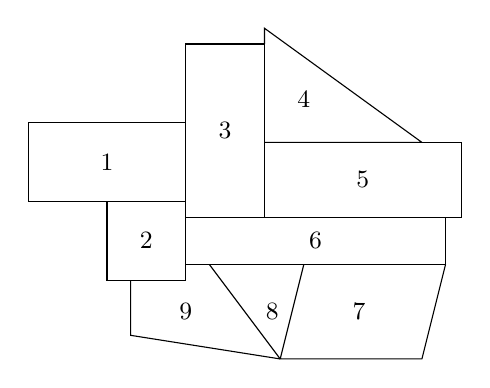
\begin{tikzpicture}[x=10mm,y=10mm, font=\small]
\draw (0,0) rectangle  (2,1) node[midway] {1};
\draw (1,-1) rectangle  (2,0) node[midway] {2};
\draw (2,-.2) rectangle  (3,2) node[midway] {3};
\draw (3,2)-- (3,2.2) -- (5,.75) --(3,.75);
\draw (3,.75) rectangle  (5.5,-.2) node[midway] {5};
\draw (2,-.2) rectangle  (5.3,-.8) node[midway] {6};
\draw (5.3,-.8) -- (5,-2) --(3.2,-2) --(3.5,-.8);
\draw (3.2,-2) -- (2.3,-.8);
\draw (3.2,-2) -- (1.3,-1.7)-- (1.3,-1);
 \node at (3.5,1.3) {4};
 \node at (4.2,-1.4) {7};
 \node at (3.1,-1.4) {8};
 \node at (2,-1.4) {9};
\end{tikzpicture}
 \caption{Esercizio \ref{ese:B.62}.}\label{fig:B.23}
\end{figure}
\end{inaccessibleblock}

% \begin{figure}[h]
% \begin{minipage}[]{1\textwidth}
%  \centering
%  % (c) 2012 Dimitrios Vrettos - d.vrettos@gmail.com

\begin{tikzpicture}[x=10mm,y=10mm, font=\small, every state/.style={draw=CornflowerBlue, minimum size=0pt}, every loop/.style={draw=Maroon}]
\draw (0,0) circle (1.5);
\node at (0,-2) {1};
\node[state] (1) at (-.6,.7) {$-12$};
\node[state] (2) at (.5,.5) {$-1$};
\node[state] (3) at (.5,-.8) {$-15$};
\node[state] (4) at (-.6,-.7) {$-7$};

\begin{scope}[->, Maroon]
 \draw (3)--(1);
 \draw (1)--(2);
 \draw (3)--(2); 
 \draw (3)--(4);
\draw (4)--(2);
 \draw (1)--(4);
\end{scope}

 \begin{scope}[xshift=31mm]
\draw (0,0) circle (1.5);
\node at (0,-2) {2};
\node[state] (1) at (-1,0) {$a$};
\node[state] (2) at (.5,.7) {$b$};
\node[state] (3) at (.5,-.5) {$c$};
\node[state] (4) at (-.6,-.7) {$m$};

\begin{scope}[->]
\path (1) edge[loop above] node{} ()
	(2) edge[loop above] node{} ()
(3) edge[loop below] node{} ()
(4) edge[loop left] node{} ();

\end{scope}
\begin{scope}[->, Maroon]
\draw (1)--(3);
\draw (1)--(2);
\draw (2)--(3);
\end{scope}
 \end{scope}

 \begin{scope}[xshift=62mm]
\draw (0,0) circle (1.5);
\node at (0,-2) {3};
\node[state] (1) at (-1,0) {$M$};
\node[state] (2) at (0,.8) {$B$};
\node[state] (3) at (1,0) {$C$};
\node[state] (4) at (0,-1) {$F$};


\begin{scope}[->]
\path (1) edge[loop above] node{} ()
	(2) edge[loop above] node{} ()
(3) edge[loop above] node{} ()
(4) edge[loop left] node{} ();

\end{scope}
\begin{scope}[->, Maroon]
\draw (1)--(2);
\draw (1)--(3);
\draw (1)--(4);
\draw (2)--(4);
\draw (4)--(3);
\end{scope}
 \end{scope}
\end{tikzpicture}
%  \caption{Esercizio \ref{ese:B.58}.}\label{fig:B.22}
% \end{minipage}
% %\hfill
% \begin{minipage}[]{\textwidth}
%  \centering
%  % (c) 2012 Dimitrios Vrettos - d.vrettos@gmail.com

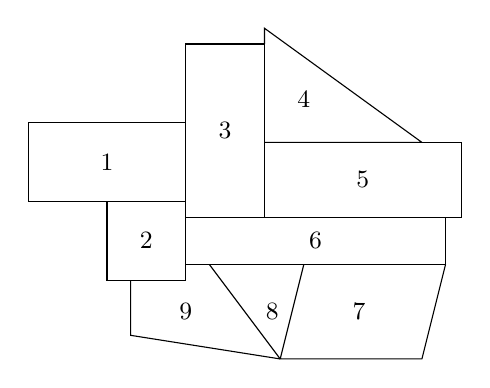
\begin{tikzpicture}[x=10mm,y=10mm, font=\small]
\draw (0,0) rectangle  (2,1) node[midway] {1};
\draw (1,-1) rectangle  (2,0) node[midway] {2};
\draw (2,-.2) rectangle  (3,2) node[midway] {3};
\draw (3,2)-- (3,2.2) -- (5,.75) --(3,.75);
\draw (3,.75) rectangle  (5.5,-.2) node[midway] {5};
\draw (2,-.2) rectangle  (5.3,-.8) node[midway] {6};
\draw (5.3,-.8) -- (5,-2) --(3.2,-2) --(3.5,-.8);
\draw (3.2,-2) -- (2.3,-.8);
\draw (3.2,-2) -- (1.3,-1.7)-- (1.3,-1);
 \node at (3.5,1.3) {4};
 \node at (4.2,-1.4) {7};
 \node at (3.1,-1.4) {8};
 \node at (2,-1.4) {9};
\end{tikzpicture}
%  \caption{Esercizio \ref{ese:B.62}.}\label{fig:B.23}
% \end{minipage}
% \end{figure}

%%%%%%%%%%%%%%%%%%%%%%%%%%%%%%%%%%%%%%%%%%%%%%%%%%%%

%\subsubsection*{D.1 - Funzioni o applicazioni}
\subsubsection*{\numnameref{sec:funzioni}}

\begin{esercizio}
 \label{ese:D.1}
 Per le funzioni rappresentate nell'esempio~\ref{ex:D.1}, completa:

 \begin{itemize*}
\item figura~a:~$\Dom =\ID = \dotfill$ $\Cod = \IM = \dotfill$ $f(a) = \dotfill$
\item figura~c:~$\Dom = \ID = \dotfill$ $\Cod = \IM = \dotfill; f(\dots)= 4$
\end{itemize*}
 \end{esercizio}

\begin{esercizio}
 \label{ese:D.2}
È vero che la corrispondenza che associa ad ogni regione italiana il suo 
capoluogo di provincia è una funzione?

\begin{enumeratea}
\item Completa:~$\Dom = \ID = \dotfill$
\item è vero che~$\IM = $\{ città d'Italia\}?
\item completa~$f$(Liguria)$=$\dotfill; $f(\dotfill) = $Cagliari?
\end{enumeratea}
\end{esercizio}

\end{comment}

\begin{esercizio}
 \label{ese:D.3}
Assegnati gli insiemi~$A=$\{mare, ruspa, fegato, generale\} 
e~$B=$\{1,2,3,4,5,6,7,8,9\} la corrispondenza
che associa ad ogni elemento di~$A$ il numero di lettere di cui è
composta la parola è una funzione?

\begin{enumeratea}
\item Rappresentala con grafico sagittale e stabilisci l'insieme immagine;
\item quale relazione sussiste tra~$B$ e~$\IM$?
\end{enumeratea}
\end{esercizio}

\begin{esercizio}
 \label{ese:D.4}
Quali tra le seguenti corrispondenze sono funzioni?
\begin{center}
 \begin{tabular}{*3{l}}
 \toprule
  Dominio & Codominio & Corrispondenza\\
\midrule
libri & autori & a ogni libro associa l'autore\\
canzoni & cantanti & a ogni canzone associa il cantante\\
portoni di una via & numeri & a ogni portone associa il numero civico\\
computer & sistemi operativi & a ogni computer associa il S.O. installato\\
\bottomrule
 \end{tabular}
\end{center}
\end{esercizio}

\begin{esercizio}
 \label{ese:D.5}
Si è ammessi alla facoltà~$U$ se nel test
d'ingresso si è avuto un punteggio compreso tra~60
incluso e~100 incluso. La corrispondenza che associa ad ogni studente
che ha superato il test il punteggio ottenuto è una funzione? Se rispondi
affermativamente, sai dire di che tipo è la funzione?
\end{esercizio}


\begin{esercizio}
 \label{ese:D.6}
Spiega perché la funzione che associa a ciascuna
persona il suo codice fiscale è biunivoca.
\end{esercizio}

%\subsubsection*{D.2 - Funzioni tra insiemi numerici}
% \subsubsection*{\numnameref{sec:D_fnumeriche}}

\begin{esercizio}
 \label{ese:D.7}
Nella corrispondenza che associa ad ogni intero il suo valore assoluto 
(esempio~\ref{ex:D.5}), è vero che scelto un qualunque numero naturale è
possibile determinare almeno un numero intero di cui è immagine?
Completate:~$f({\ldots}{\ldots}) = 45.$
L'osservazione precedente permette di concludere che
tale funzione è suriettiva?
Fate la rappresentazione sagittale della funzione.
\end{esercizio}

\begin{esercizio}
 \label{ese:D.10}
Consideriamo la funzione~$f$ che associa ad ogni numero razionale il suo triplo.

$Q\overset{{f}}{{\rightarrow }}Q$ la sua espressione in forma
analitica è~$f: y = {\dots}{\dots}{\dots}$

$\Dom = \ID = \insQ$ possiamo moltiplicare per~3 qualunque numero razionale.

$\Cod = \IM =\insQ$ infatti per ogni numero razionale $y$ c'è un numero 
razionale $x$ di cui $y$ è il triplo, basta dividere $y$ per 3.
%il triplo di un numero razionale è ancora un numero razionale.
%
%Rispondete:
\vspace{-6pt}
\begin{enumeratea}
\item qual è l'immagine di~0?\dotfill
\item quale elemento del dominio ha per immagine~5?\dotfill
\item è vero che ogni numero positivo ha l'immagine positiva?\dotfill
\item è vero che~$-1$ è immagine di~$-3$?\dotfill
\item la funzione è iniettiva?
\item la funzione è biunivoca?
\end{enumeratea}
% Fa il grafo sagittale della funzione.
\end{esercizio}

\newpage %---------------------------------------------------

\begin{esercizio}
 \label{ese:D.11}
Per ciascuna delle seguenti funzioni determinare l'insieme di definizione, 
l'insieme
immagine e stabilire se la funzione è iniettiva o suriettiva.
\begin{multicols}{3}
\begin{enumeratea}
\item $y:\insN\rightarrow\insN;\quad x \rightarrow 2x$
\item $y:\insN\rightarrow\insN;\quad x \rightarrow \frac{1}{x}$
\item $y:\insZ\rightarrow\insZ;\quad x \rightarrow 2x$
\item $y:\insZ\rightarrow\insZ;\quad x \rightarrow x^{2}$
\item $y:\insQ\rightarrow\insQ;\quad x \rightarrow 2x$
\item $y:\insQ\rightarrow\insQ;\quad x \rightarrow \frac{1}{x}$
\end{enumeratea}
\end{multicols}
\end{esercizio}

\begin{comment}

\begin{esercizio}
 \label{ese:D.8}
Data la funzione~$y=x-2$ con dominio~$\insN-\{0,1\}$ e codomino~$\insN$ 
completa 
l'analisi dell'esempio~\ref{ex:D.7}
\begin{enumeratea}
\item elementi diversi del dominio hanno immagini diverse, quindi tale funzione 
è \emph{iniettiva};
si ha anche~$\Cod=\IM = \insN$ e pertanto la funzione è \emph{suriettiva}, 
quindi \dotfill;
\item preso~$y = 8$ sapresti trovare l'elemento del dominio di cui è immagine? 
\dotfill;
\end{enumeratea}
\end{esercizio}

\begin{esercizio}
 \label{ese:D.9}
Stabilisci se la funzione~$f:y=\frac{1}{x}$ è
iniettiva. Nell'insieme immagine c'è lo zero?

Completate~$\Cod = \IM =\ldots$
Completate la tabella
\begin{center}
\begin{tabular}{l*8{c}}
\toprule
$x\in \insQ_{0}$ & $-2$ & $-7/8$ & $+1$ & & & & $-1$ & \\
$y\in \insQ_{0}$ & & & & $+1/3$ & $-12/5$ & $-7/8$ & & $-1$\\
\bottomrule
\end{tabular}
\end{center}
\end{esercizio}

\begin{esercizio}
 \label{ese:D.12}
Per ciascuna delle funzioni elencate in~$\insR \times\insR$, riempite le colonne 
della tabella.
\begin{center}
\begin{tabular}{l*2{c}}
\toprule
$y=f(x)$ & $f(x)$ è iniettiva? & $x=f^{-1}(y)$\\
\midrule
$y=2x$ & & \\
$y=x+2$ & & \\
$y=2x-2$ & & \\
$y=x^{2}$ & & \\
$y=\frac{1}{2}x-\frac{5}{2}$ & & \\
$y=\sqrt{2}\cdot x$ & & \\
\bottomrule
\end{tabular}
\end{center}
\end{esercizio}

\begin{esercizio}
 \label{ese:D.13}
Assegnata la funzione lineare~$f:y=m\cdot x+q$, essendo una funzione
iniettiva la sua inversa è:\dotfill
\end{esercizio}

\begin{esercizio}
 \label{ese:D.14}
Date le funzioni~$f(x)=2x+1$ e~$g(x)=3x+2$ che hanno per dominio
rispettivamente~$A=\left\{x\in \insZ/-2\le x\le~2\right\}$,
$B=\left\{x\in \insZ\text{/}-1\le x\le~3\right\}$
Scrivi le espressioni analitiche delle funzioni~$f\circ g$ e~$g\circ f$
\end{esercizio}

%\subsubsection*{D.4 - La retta e gli insiemi numerici}
% \subsubsection*{\numnameref{sec:D_retta}}

\end{comment}

\begin{esercizio}
\label{ese:D.15}
Determina sulla retta reale i punti immagine dei seguenti numeri reali:~$\alpha 
=\frac{3}{2}\sqrt{2}$\, $\beta =\frac{2}{5}+\frac{1}{\sqrt{2}}$
\, $\delta =-\left(\sqrt{3}+\sqrt{2}\right)$\, $\lambda =\sqrt{3}-3$
\end{esercizio}

% \begin{esercizio}
% \label{ese:D.16}
% Verifica che il numero~$\chi =\sqrt{3}+\sqrt{2}$ non è uguale al numero~$\omega 
% =\sqrt{5}$, usando la rappresentazione sulla retta orientata.
% \end{esercizio}

\begin{esercizio}
\label{ese:D.17}
Stabilisci il valore di verità della proposizione: ``poiché tra~$2$ e~$3$ non vi 
è nessun altro numero naturale, anche tra~$\sqrt{2}$ e
$\sqrt{3}$ non vi è nessun numero reale''.
\end{esercizio}

%\subsubsection*{D.6 - Il grafico di una funzione}
% \subsubsection*{\numnameref{sec:D_grafico}}

\begin{esercizio}
\label{ese:D.37}
Per ognuna delle seguenti funzioni compila una tabella di valori e 
rappresentala in un piano cartesiano.

 $f_1:\insQ \rightarrow \insQ\quad y=\dfrac{1}{2}x$ \quad
 $f_2:\insQ \rightarrow \insQ\quad y=-x$ \quad
 $f_3:\insQ \rightarrow \insQ\quad y=2-3x$
\end{esercizio}

\begin{esercizio}
\label{ese:D.38}
Esprimi con linguaggio comune la funzione~$f_1$ dell'esercizio precedente e 
rispondi alle domande:

\begin{enumeratea}
\item qual è l'immagine di~$0$?  $y=\ldots \ldots $
\item quale elemento del dominio ha per immagine~$5$? $x=\ldots \ldots $
\item è vero che ogni numero positivo ha l'immagine positiva? Perché?
\item è vero che~$-1$ è immagine di~$-2$? Perché?
\end{enumeratea}
\end{esercizio}

\begin{esercizio}
\label{ese:D.39}
Dopo aver determinato per ciascuna delle seguenti funzioni il coefficiente 
angolare~$k$, tracciane il grafico in un riferimento cartesiano ortogonale:
\begin{multicols}{3}
 \begin{enumeratea}
\item $f_{1}:\, y=\frac{1}{2}x$
\item $f_{2}:\, y=x$
\item $f_{3}:\, y=\frac{4}{3}x$
\item $f_{4}:\, y=\frac{3}{5}x$
\item $f_{5}:\, y=5x$
\item $f_{6}:\, y=-{\frac{1}{2}}x$
\item $f_{7}:\, y=-x$
\item $f_{8}:\, y=-{\frac{3}{4}}x$
\end{enumeratea}
\end{multicols}
\end{esercizio}

\begin{esercizio}
\label{ese:D.40}
Riporta in uno stesso riferimento cartesiano ortogonale le prime cinque funzioni 
dell'esercizio precedente.
Evidenzia con un colore diverso la funzione~$f_2$, calcola poi il coefficiente 
angolare~$m$ compilando la seguente tabella:
\begin{center}
 \begin{tabular}{cccccc}
  \toprule
  $\quad f \quad $ & $ \quad f_1 \quad $ & $ \quad f_2 \quad $ & $ \quad f_3 
\quad $ & $ \quad f_4 \quad $ & $ \quad f_5 \quad $\\
  $m$ & & & & &\\
  \bottomrule
 \end{tabular}
\end{center}

\emph{Cancella i termini errati} nella seguente analisi:
``Tutte le funzioni hanno coefficiente angolare positivo/negativo; tutte le 
rette formano con l'asse orientato delle~$x$ un angolo ottuso/acuto;
tutte le rette aventi coefficiente minore di~$1$ stanno sopra/sotto la~$f_{2}$ 
tutte le rette aventi coefficiente maggiore di~$1$
stanno sopra/sotto la~$f_{2}$''.
\end{esercizio}

\begin{esercizio}
\label{ese:D.41}
Ripeti l'esercizio precedente per le altre tre funzioni, evidenziando la 
funzione~$f_{7}$ costruisci l'analoga tabella e
\emph{cancella i termini errati} nella seguente analisi:
``Tutte le funzioni hanno coefficiente angolare positivo/negativo; tutte le 
rette formano con l'asse orientato delle~$x$ un angolo ottuso/acuto;
tutte le rette aventi coefficiente minore di~$-1$ stanno sopra/sotto la~$f_{7}$ 
tutte le rette aventi coefficiente maggiore di~$-1$
stanno sopra/sotto la~$f_{7}$''.
\end{esercizio}

\begin{esercizio}
\label{ese:D.42}
Se~$x$ rappresenta la misura del lato di un triangolo equilatero; determina la 
misura della altezza al variare della misura del lato.
Nel riferimento cartesiano ortogonale traccia il grafico della funzione 
ottenuta.
\end{esercizio}

% \begin{esercizio}
% \label{ese:D.43}
% Quale deve essere la misura del lato di un quadrato per avere la diagonale 
% di~$2\unit{m}$?
% \end{esercizio}

% \begin{esercizio}
% \label{ese:D.44}
% Traccia nel riferimento cartesiano ortogonale il grafico delle 
% funzioni:~$y=-2$\, $y=6$\, $y=0$\, $y=-1$\, $y=3$
% \end{esercizio}

\begin{esercizio}
\label{ese:D.45}
Traccia nel riferimento cartesiano la funzione~$y=1$ e~$y=-3$ nello stesso 
riferimento traccia la funzione~$y=2x$
Le tre rette individuano nel piano due punti. Determina la distanza dei due 
punti.
\end{esercizio}

\begin{esercizio}
\label{ese:D.46}
Le due funzioni~$f_{1}$ e~$f_{2}$ di proporzionalità diretta assegnate dalle 
tabelle seguenti delimitano sulla funzione~$y=-2$
un segmento; determina la misura del segmento e il suo punto medio:
 \begin{center}
 \begin{tabular}{cccccc}
  \toprule
  \multirow{2}*{$f_1$} &$x$&$-2$& $0$ & $3$ &$-1$\\
             &$y$&$2$& $0$ & $-3$ &$1$\\
  \midrule
  \multirow{2}*{$f_2$} &$x$&$1$& $0$ & $3$ &$-2$\\
             &$y$&$4$& $0$ & $12$ &$-8$\\
  \bottomrule
 \end{tabular}
 \end{center}

\end{esercizio}

\begin{esercizio}
\label{ese:D.47}
Traccia il grafico cartesiano delle funzioni~$f_{1}:\,y=2x$, 
$f_{2}:\,y=-{\frac{1}{2}}x$, $f_{3}:\,y=2$ e indica con~$A$ e~$B$
rispettivamente i punti di intersezione di~$f_{1}$ con~$f_{3}$ e di~$f_{2}$ 
con~$f_{3}$
Considera il triangolo~${AOB}$ ($O$ è l'origine del riferimento). È vero 
che~$\overline{AB}^{2}=\overline{AO}^{2}+\overline{OB}^{2}$?
Sai trarre una caratteristica del triangolo~${AOB}$? Traccia nello stesso 
riferimento la funzione~$f_{4}:\,y-4$ e indica con
$C$ e~$D$ rispettivamente i punti di intersezione di~$f_{1}$ con~$f_{4}$ e 
di~$f_{2}$ con~$f_{4}$ Calcola l'area del quadrilatero~${ABCD}$
\end{esercizio}

\begin{esercizio}
\label{ese:D.48}
Sono assegnate le funzioni lineari:~$f_{1}:\,y=\frac{1}{2}x-2$, 
$f_{2}:\,y=-x-\frac{3}{4}$, $f_{3}:\,y=6x-6$
Rappresentale in un riferimento cartesiano ortogonale dopo aver compilato per 
ciascuna una tabella di valori.
\end{esercizio}

\begin{esercizio}
\label{ese:D.49}
Segna nel riferimento cartesiano ortogonale i punti assegnati tramite la 
tabella:
\begin{center}
 \begin{tabular}{cccccc}
  \toprule
  $x$ &$-3$&$-3/2$& $0$ & $3$ &$6$\\
  $y$ & $-2$ & $-1$ & $0$ & $2$ & $4$\\
  \bottomrule
 \end{tabular}
\end{center}

La funzione assegnata è una proporzionalità diretta?

Scrivi la formula~$y=\ldots \ldots \ldots$

Completa ora la tabella avente i medesimi valori della variabile indipendente, 
ma i valori della variabile dipendente siano ottenuti
dai precedenti diminuiti di~$2$:
\begin{center}
 \begin{tabular}{cccccc}
  \toprule
  $x$ &$ \quad -3 \quad $ & $ \quad -3/2 \quad $ & $ \quad 0 \quad $ & $ \quad 3 
\quad $ & $ \quad 6 \quad $\\
  $y$ &  &  & $-2$ &  & \\
  \bottomrule
 \end{tabular}
\end{center}

Scrivi la formula della nuova funzione~$y=\ldots \ldots \ldots$

Traccia il suo grafico nello stesso riferimento. È una funzione lineare?
\end{esercizio}

\begin{esercizio}
\label{ese:D.50}
La tabella individua coppie di punti allineati; trova la formula che descrive 
ciascuna funzione lineare e traccia il suo grafico:\quad
\begin{center}
 \begin{tabular}{ccccccc}
  \toprule
  \multirow{2}*{$f_1$} &$x$&$5$& $-1$ & $0$ &$3$&$1$\\
             &$y$&$-2$& $4$ & $-3$ &$0$&$2$\\
  \midrule
  \multirow{2}*{$f_2$} &$x$&$-4$& $-4/3$ & $0$ &$-1/3$&$4/3$\\
             &$y$&$-2$& $0$ & $1$ &$3/4$&$2$\\
  \midrule
  \multirow{2}*{$f_3$} &$x$&$-6$& $-1$ & $0$ &$3$&$1$\\
             &$y$&$-11/3$& $-1/3$ & $1/3$ &$7/3$&$1$\\
  \bottomrule
 \end{tabular}
\end{center}
\end{esercizio}

\begin{esercizio}
\label{ese:D.51}
Traccia il grafico delle seguenti funzioni di proporzionalità inversa:
\begin{multicols}{3}
 \begin{enumeratea}
\item $f_{1}:\, y=-{\frac{3}{2x}}$
\item $f_{2}:\, y=\frac{1}{x}$
\item $f_{3}:\, y=\frac{5}{x}$
\item $f_{4}:\, y=\frac{-3}{x}$
\item $f_{5}:\, y=-{\frac{1}{x}}$
\item $f_{6}:\, y=-\frac{2}{5x}$
\end{enumeratea}
\end{multicols}
\end{esercizio}

\begin{esercizio}
\label{ese:D.52}
Traccia nelle stesso riferimento cartesiano ortogonale la curva~$\gamma:\, 
y=-{\frac{1}{2x}}$ e le rette~$r_{1}:\, y=2$ e
$r_{2}:\, y=-2$ Verifica che l'origine del riferimento è il punto medio del 
segmento avente per estremi i punti
$A_{1}=r_{1}\cap \gamma$ e~$A_{2}=r_{2}\cap \gamma$
\end{esercizio}

\begin{esercizio}
\label{ese:D.53}
Traccia il grafico delle seguenti funzioni di proporzionalità quadratica:
\begin{multicols}{3}
 \begin{enumeratea}
\item $f_{1}:\, y=-x^{2}$
\item $f_{2}:\, y=x^{2}$
\item $f_{3}:\, y=-{\frac{1}{2}}x^{2}$
\item $f_{4}:\, y=-{\frac{5}{2}}x^{2}$
\item $f_{5}:\, y=\frac{3}{4}x^{2}$
\item $f_{6}:\, y=\frac{7}{3}x^{2}$
\end{enumeratea}
\end{multicols}
\end{esercizio}

\begin{esercizio}
\label{ese:D.54}
Dai grafici dell'esercizio precedente trai le conclusioni, completando.
\begin{enumeratea}
\item se~$k>0$ allora i punti della parabola si trovano~$\ldots \ldots \ldots$
\item se~$k<0$ allora i punti della parabola si trovano~$\ldots \ldots \ldots$
\item se~$k>1$ allora la curva è più aperta o più chiusa rispetto 
alla~$y=x^{2}$? $\ldots \ldots \ldots$
\item se~$0<k<1$ allora la curva è più aperta o più chiusa rispetto alla  
$y=x^{2}$? $\ldots \ldots \ldots$
\item se~$k<-1$ allora la curva è più aperta o più chiusa rispetto alla  
$y=-x^{2}$? $\ldots \ldots \ldots$
\item se~$-1<k<0$ allora la curva è più aperta o più chiusa rispetto alla  
$y=-x^{2}$? $\ldots \ldots \ldots$
\end{enumeratea}
\end{esercizio}

\begin{esercizio}
\label{ese:D.55}
Determina la distanza del punto di ascissa~$x=-2$ della parabola~$y=3x^{2}$ dal 
suo vertice.
\end{esercizio}

\begin{esercizio}
\label{ese:D.56}
Sono assegnate le funzioni~$f_{1}:\, y=(-x)^{2}$ e~$f_{2}:\, y=-x^{2}$ di 
proporzionalità quadratica.
Spiega se e perché sono o non sono la stessa funzione.
Danne di ciascuna la descrizione in linguaggio comune.
Costruisci per ciascuna una tabella di valori e costruisci il rispettivo 
grafico.
Puoi confermare la risposta data alla prima richiesta?
\end{esercizio}

\begin{esercizio}
\label{ese:D.57}
Completa la seguente tabella:
\begin{center}
 \begin{tabular}{llll}
  \toprule
  Funzione&In linguaggio comune&Formula&Tipo\\
  $f_1$&Associa ad ogni~$x$ reale il valore~$-2/3$& &\\
  $f_2$&Associa ad ogni~$x$ reale il triplo del suo quadrato& & \\
  $f_3$& &$y=-5x^2$& \\
  $f_4$&Associa ad ogni~$x$ reale il suo doppio aumentato di~$3/2$& & \\
  $f_5$&Associa ad ogni~$x$ reale~$\neq~0$ l'opposto del suo reciproco& & \\
  $f_3$& &$y=-5x$& \\
  \bottomrule
 \end{tabular}
\end{center}
Traccia nel riferimento cartesiano ortogonale le funzioni assegnate. Per quale/i 
è vero che per qualunque~$x$ del dominio è~$\IM=\insR$?
\end{esercizio}

% \begin{esercizio}
% \label{ese:D.58}
% Il rettangolo~${ABCD}$ ha il lato~${AB}$ triplo del lato~${BC}$ 
% Indica~$\overline{BC}=x$ determina il perimetro del
% rettangolo in funzione di~$x$  $2p=\ldots \ldots \ldots$
% Spiega perché è necessaria la condizione~$x>0$ rappresenta graficamente nel 
% riferimento cartesiano la funzione perimetro.
% Determina ora l'area in funzione di~$x$, $\Area=\ldots \ldots \ldots$ 
% rappresenta la funzione area, nello stesso riferimento.
% \end{esercizio}
% 
% \begin{esercizio}
% \label{ese:D.59}
% Il triangolo rettangolo~${ABC}$, retto in~$A$ ha i cateti l'uno doppio 
% dell'altro. Indica la misura del cateto minore~$\overline{AB}=x$
% e spiega perché è necessaria la condizione~$x>0$
% 
% Determina in funzione di~$x$ l'area del triangolo. $\Area=\ldots \ldots \ldots$
% rappresenta questa funzione nel riferimento cartesiano ortogonale.
% Stabilisci le misure dei cateti se l'area è di~$20\unit{cm^2}$
% 
% Calcola in funzione di~$x$ il perimetro del triangolo:~$2p=\ldots \ldots 
% \ldots$, rappresenta come varia la funzione perimetro al variare di~$x$
% \end{esercizio}

\begin{esercizio}
\label{ese:D.60}
Nel triangolo isoscele~${ABC}$ il lato obliquo~${AB}$ è doppio della base~${BC}$ 
indica~$\overline{BC}=x$ e determina in funzione
di~$x$ il perimetro del triangolo. $2p=\ldots \ldots \ldots$
Di che funzione si tratta? Descrivila e rappresentala nel riferimento cartesiano 
ortogonale, dopo aver fissato le opportune condizioni
sulla variabile indipendente.

Se il perimetro è~$120\unit{cm}$, quanto misurano i lati del triangolo?
Calcola, in questo caso, l'area del triangolo e la misura delle altezze relative 
ai lati uguali.
\end{esercizio}

\begin{esercizio}
\label{ese:D.61}
Traccia il grafico della funzione
\[f(x)=\left\{\begin{array}{l}
y=-1\text{ se } x>1\\
y=2x\text{ se } x \le~1\end{array}\right..\]
\end{esercizio}

\begin{esercizio}
\label{ese:D.62}
Traccia il grafico della funzione~$y=|{x+1}|$
\end{esercizio}

\begin{esercizio}
\label{ese:D.63}
Un caseificio vende mozzarelle a \officialeuro\ $4,50$ al chilo ai clienti che 
acquistano fino~$10\unit{kg}$ di mozzarella, per i clienti che
fanno acquisti superiori ai~$10\unit{kg}$ vende a \officialeuro\ $4,00$ al kg 
per la parte che eccede i~$10\unit{kg}$ e per i primi~$10\unit{kg}$
vende sempre a \officialeuro\ $4,50$ Per i clienti dei grandi supermercati che 
acquistano quantità superiori a~$100\unit{kg}$ vende a \officialeuro\ $3,50$
al kg. Codifica con opportune formule la funzione costo:

\[\left\{\begin{array}{l}
\ldots\ldots\ldots \text{ se } x \le~10\\
\ldots\ldots\ldots \text{ se } 10< x \le~100\\
\ldots\ldots\ldots \text{ se } x > 100\end{array}\right..
\]
Determina il costo dei seguenti ordini:
\begin{center}
 \begin{tabular}{cccccccc}
  \toprule
  $\unit{kg}$ & $ \quad 3,5 \quad $ & $ \quad 11,8 \quad $ & $ \quad 78 \quad $ 
& $ \quad 120 
\quad $ & & &\\
  euro& & & & & $ \quad 360 \quad $ & $ \quad 57 \quad $ & $ \quad 35 \quad $\\
  \bottomrule
 \end{tabular}
\end{center}

Rappresenta graficamente la funzione.
\end{esercizio}

\begin{esercizio}
\label{ese:D.64}
Dal grafico della funzione stabilisci insieme di definizione~$\Dom$, insieme 
immagine~$\IM$, verifica se la funzione è iniettiva, suriettiva o biettiva.
\begin{center}
 % (c) 2012 Dimitrios Vrettos - d.vrettos@gmail.com
\begin{tikzpicture}[x=7mm, y=7mm, scale=.8]
  \tkzInit[xmin=-3.5,xmax=3.3,ymin=-2.5,ymax=2]
  \clip (-3.5,-3) rectangle (21,3);

    \tkzDrawY[noticks]
    \tkzDrawX[noticks]

  \tkzFct[domain=-3*pi/2:3*pi/2,thick,color=Maroon]{sin(-x)*2}

\begin{scope}[xshift=59mm]
    \tkzDrawY[noticks]
    \tkzDrawX[noticks]

  \tkzFct[domain=0:3.5,thick,color=Maroon]{5*x/12+.5}
  \tkzFct[domain=-3.5:0,thick,color=Maroon]{5*x/12-.8}
\end{scope}

\begin{scope}[xshift=118mm]
    \tkzDrawY[noticks]
    \tkzDrawX[noticks]

  \tkzFct[domain=-3.5:3.5,thick,color=Maroon]{x*x-2}
\end{scope}
\end{tikzpicture}
\end{center}

\end{esercizio}

%%%%%%%%%%%%%%%%%%%%%%%%%%%%%%%%%%%%%%%%%%%%%%%%%%
